\documentclass[conference]{IEEEtran}
\IEEEoverridecommandlockouts
% The preceding line is only needed to identify funding in the first footnote. If that is unneeded, please comment it out.
% \usepackage{hyperref}
\usepackage{url}
% \usepackage[hyphens]{url}
% \usepackage{breakurl}
% \usepackage[bookmarks=false,hidelinks]{hyperref} 

\usepackage{cite}
\usepackage{amsmath,amssymb,amsfonts}
\usepackage{graphicx}
\usepackage{textcomp}
\usepackage{algorithm}
\usepackage{algpseudocode}
\usepackage{graphicx}

\usepackage{xcolor}
\usepackage{lipsum,framed}
\def\BibTeX{{\rm 
B\kern-.05em{\sc 
i\kern-.025em b}
\kern-.08em
    T\kern-.1667em\lower.7ex\hbox{E}\kern-.125emX}}


   
\begin{document}

% \title{Option Batch-Shuffle Trick: Answering MCQs on Telecommunication Documents using Large Language Models*\\
% {\footnotesize \textsuperscript{*}Note: Sub-titles are not captured in Xplore and
% should not be used}
% % \thanks{Identify applicable funding agency here. If none, delete this.}
% }

\title{AmaSQuAD: A Benchmark for Amharic Extractive Question Answering\\
}



\author{
\IEEEauthorblockN{Nebiyou Daniel Hailemariam, Blessed Guda, Tsegazeab Tefferi, }
\IEEEauthorblockA{\textit{College of Engineering, Carnegie Mellon University} \\
% Kigali, Rwanda (Blessed Guda, Gabrial Zencha A., Lawrence Francis) \\
% Pittsburgh, USA (Carlee Joe-Wong) \\
nhailema@alumni.cmu.edu, blessed@alumni.cmu.edu, ttefferi@alumni.cmu.edu
}

}


\maketitle
\begin{abstract}  
Test time scaling is currently one of the most active research areas that shows promise after training time scaling has reached its limits.
Deep-thinking (DT) models are a class of recurrent models that can perform easy-to-hard generalization by assigning more compute to harder test samples.
However, due to their inability to determine the complexity of a test sample, DT models have to use a large amount of computation for both easy and hard test samples.
Excessive test time computation is wasteful and can cause the ``overthinking'' problem where more test time computation leads to worse results.
In this paper, we introduce a test time training method for determining the optimal amount of computation needed for each sample during test time.
We also propose Conv-LiGRU, a novel recurrent architecture for efficient and robust visual reasoning. 
Extensive experiments demonstrate that Conv-LiGRU is more stable than DT, effectively mitigates the ``overthinking'' phenomenon, and achieves superior accuracy.
\end{abstract}  

\section{Introduction}
\label{sec:introduction}
The business processes of organizations are experiencing ever-increasing complexity due to the large amount of data, high number of users, and high-tech devices involved \cite{martin2021pmopportunitieschallenges, beerepoot2023biggestbpmproblems}. This complexity may cause business processes to deviate from normal control flow due to unforeseen and disruptive anomalies \cite{adams2023proceddsriftdetection}. These control-flow anomalies manifest as unknown, skipped, and wrongly-ordered activities in the traces of event logs monitored from the execution of business processes \cite{ko2023adsystematicreview}. For the sake of clarity, let us consider an illustrative example of such anomalies. Figure \ref{FP_ANOMALIES} shows a so-called event log footprint, which captures the control flow relations of four activities of a hypothetical event log. In particular, this footprint captures the control-flow relations between activities \texttt{a}, \texttt{b}, \texttt{c} and \texttt{d}. These are the causal ($\rightarrow$) relation, concurrent ($\parallel$) relation, and other ($\#$) relations such as exclusivity or non-local dependency \cite{aalst2022pmhandbook}. In addition, on the right are six traces, of which five exhibit skipped, wrongly-ordered and unknown control-flow anomalies. For example, $\langle$\texttt{a b d}$\rangle$ has a skipped activity, which is \texttt{c}. Because of this skipped activity, the control-flow relation \texttt{b}$\,\#\,$\texttt{d} is violated, since \texttt{d} directly follows \texttt{b} in the anomalous trace.
\begin{figure}[!t]
\centering
\includegraphics[width=0.9\columnwidth]{images/FP_ANOMALIES.png}
\caption{An example event log footprint with six traces, of which five exhibit control-flow anomalies.}
\label{FP_ANOMALIES}
\end{figure}

\subsection{Control-flow anomaly detection}
Control-flow anomaly detection techniques aim to characterize the normal control flow from event logs and verify whether these deviations occur in new event logs \cite{ko2023adsystematicreview}. To develop control-flow anomaly detection techniques, \revision{process mining} has seen widespread adoption owing to process discovery and \revision{conformance checking}. On the one hand, process discovery is a set of algorithms that encode control-flow relations as a set of model elements and constraints according to a given modeling formalism \cite{aalst2022pmhandbook}; hereafter, we refer to the Petri net, a widespread modeling formalism. On the other hand, \revision{conformance checking} is an explainable set of algorithms that allows linking any deviations with the reference Petri net and providing the fitness measure, namely a measure of how much the Petri net fits the new event log \cite{aalst2022pmhandbook}. Many control-flow anomaly detection techniques based on \revision{conformance checking} (hereafter, \revision{conformance checking}-based techniques) use the fitness measure to determine whether an event log is anomalous \cite{bezerra2009pmad, bezerra2013adlogspais, myers2018icsadpm, pecchia2020applicationfailuresanalysispm}. 

The scientific literature also includes many \revision{conformance checking}-independent techniques for control-flow anomaly detection that combine specific types of trace encodings with machine/deep learning \cite{ko2023adsystematicreview, tavares2023pmtraceencoding}. Whereas these techniques are very effective, their explainability is challenging due to both the type of trace encoding employed and the machine/deep learning model used \cite{rawal2022trustworthyaiadvances,li2023explainablead}. Hence, in the following, we focus on the shortcomings of \revision{conformance checking}-based techniques to investigate whether it is possible to support the development of competitive control-flow anomaly detection techniques while maintaining the explainable nature of \revision{conformance checking}.
\begin{figure}[!t]
\centering
\includegraphics[width=\columnwidth]{images/HIGH_LEVEL_VIEW.png}
\caption{A high-level view of the proposed framework for combining \revision{process mining}-based feature extraction with dimensionality reduction for control-flow anomaly detection.}
\label{HIGH_LEVEL_VIEW}
\end{figure}

\subsection{Shortcomings of \revision{conformance checking}-based techniques}
Unfortunately, the detection effectiveness of \revision{conformance checking}-based techniques is affected by noisy data and low-quality Petri nets, which may be due to human errors in the modeling process or representational bias of process discovery algorithms \cite{bezerra2013adlogspais, pecchia2020applicationfailuresanalysispm, aalst2016pm}. Specifically, on the one hand, noisy data may introduce infrequent and deceptive control-flow relations that may result in inconsistent fitness measures, whereas, on the other hand, checking event logs against a low-quality Petri net could lead to an unreliable distribution of fitness measures. Nonetheless, such Petri nets can still be used as references to obtain insightful information for \revision{process mining}-based feature extraction, supporting the development of competitive and explainable \revision{conformance checking}-based techniques for control-flow anomaly detection despite the problems above. For example, a few works outline that token-based \revision{conformance checking} can be used for \revision{process mining}-based feature extraction to build tabular data and develop effective \revision{conformance checking}-based techniques for control-flow anomaly detection \cite{singh2022lapmsh, debenedictis2023dtadiiot}. However, to the best of our knowledge, the scientific literature lacks a structured proposal for \revision{process mining}-based feature extraction using the state-of-the-art \revision{conformance checking} variant, namely alignment-based \revision{conformance checking}.

\subsection{Contributions}
We propose a novel \revision{process mining}-based feature extraction approach with alignment-based \revision{conformance checking}. This variant aligns the deviating control flow with a reference Petri net; the resulting alignment can be inspected to extract additional statistics such as the number of times a given activity caused mismatches \cite{aalst2022pmhandbook}. We integrate this approach into a flexible and explainable framework for developing techniques for control-flow anomaly detection. The framework combines \revision{process mining}-based feature extraction and dimensionality reduction to handle high-dimensional feature sets, achieve detection effectiveness, and support explainability. Notably, in addition to our proposed \revision{process mining}-based feature extraction approach, the framework allows employing other approaches, enabling a fair comparison of multiple \revision{conformance checking}-based and \revision{conformance checking}-independent techniques for control-flow anomaly detection. Figure \ref{HIGH_LEVEL_VIEW} shows a high-level view of the framework. Business processes are monitored, and event logs obtained from the database of information systems. Subsequently, \revision{process mining}-based feature extraction is applied to these event logs and tabular data input to dimensionality reduction to identify control-flow anomalies. We apply several \revision{conformance checking}-based and \revision{conformance checking}-independent framework techniques to publicly available datasets, simulated data of a case study from railways, and real-world data of a case study from healthcare. We show that the framework techniques implementing our approach outperform the baseline \revision{conformance checking}-based techniques while maintaining the explainable nature of \revision{conformance checking}.

In summary, the contributions of this paper are as follows.
\begin{itemize}
    \item{
        A novel \revision{process mining}-based feature extraction approach to support the development of competitive and explainable \revision{conformance checking}-based techniques for control-flow anomaly detection.
    }
    \item{
        A flexible and explainable framework for developing techniques for control-flow anomaly detection using \revision{process mining}-based feature extraction and dimensionality reduction.
    }
    \item{
        Application to synthetic and real-world datasets of several \revision{conformance checking}-based and \revision{conformance checking}-independent framework techniques, evaluating their detection effectiveness and explainability.
    }
\end{itemize}

The rest of the paper is organized as follows.
\begin{itemize}
    \item Section \ref{sec:related_work} reviews the existing techniques for control-flow anomaly detection, categorizing them into \revision{conformance checking}-based and \revision{conformance checking}-independent techniques.
    \item Section \ref{sec:abccfe} provides the preliminaries of \revision{process mining} to establish the notation used throughout the paper, and delves into the details of the proposed \revision{process mining}-based feature extraction approach with alignment-based \revision{conformance checking}.
    \item Section \ref{sec:framework} describes the framework for developing \revision{conformance checking}-based and \revision{conformance checking}-independent techniques for control-flow anomaly detection that combine \revision{process mining}-based feature extraction and dimensionality reduction.
    \item Section \ref{sec:evaluation} presents the experiments conducted with multiple framework and baseline techniques using data from publicly available datasets and case studies.
    \item Section \ref{sec:conclusions} draws the conclusions and presents future work.
\end{itemize}

\section{Related Work}
\label{sec:related}
FL has emerged as a crucial learning scheme for distributed training that aims to preserve user data privacy. 
However, research has uncovered various privacy vulnerabilities in FL, particularly in the form of MIA and LDIA.
This section discusses relevant works that highlight these threats in both FL and FD settings, and contextualize our research within this landscape.

\BfPara{MIA and LDIA} 
Shokri \etal~\cite{shokri2017membership} pioneered MIA research by demonstrating how model output confidence scores could reveal training data membership. 
Nasr \etal~\cite{nasr2019comprehensive} extended this to FL, showing how both passive and active adversaries could exploit gradients and model updates.
LDIA represents another significant privacy threat in FL.
Gu \etal~\cite{gu2023ldia} introduced LDIA as a new attack vector where adversaries infer label distributions from model updates. Wainakh \etal~\cite{wainakh2021user} further explored user-level label leakage through gradient-based attacks in FL.
Recent works have exposed the vulnerability of FD to inference attacks.
Yang \etal~\cite{yang2022fd} proposed FD-Leaks for performing MIA in FD settings through logit analysis. Liu \etal~\cite{liu2023mia} and Wang \etal~\cite{wang2024graddiff} enhanced MIA using shadow models via respective approaches MIA-FedDL and GradDiff, though their assumptions were limited to homogeneous environments.

\iffalse
The study of MIA in ML models was pioneered by Shokri \etal~\cite{shokri2017membership}.
They demonstrated how adversaries could exploit model output confidence scores to infer whether a specific data point was used in training.
This seminal work laid the foundation for subsequent research into privacy vulnerabilities in various ML paradigms, including FL.
Building on this, Nasr \etal~\cite{nasr2019comprehensive} extended the concept to FL environments, introducing white-box MIAs.
Their privacy analysis demonstrated how both passive and active adversaries could exploit gradients and model updates to infer private information.
\BfPara{LDIA in FL} 
LDIA represents another significant privacy threat in FL.
Gu \etal~\cite{gu2023ldia} introduced LDIA as a new attack vector, where adversaries seek to infer the distribution of labels in clients' training data by analyzing model updates.
This work showed that even when individual data points are protected, the overall data distribution might still be exposed, leading to privacy concerns.
Wainakh \etal~\cite{wainakh2021user} further explored user-level label leakage by performing gradient-based attacks in FL.

\BfPara{LDIA and MIA in FD} 
% FD has been proposed as a lightweight alternative to traditional FL.
% It reduces communication overhead by exchanging logits or softmax values instead of model parameters.
Yang \etal~\cite{yang2022fd} proposed FD-Leaks, an attack designed to perform MIA in FD settings.
By analyzing logits, adversaries can infer membership information, potentially revealing sensitive training data.
Similarly, Liu \etal~\cite{liu2023mia} presented MIA-FedDL, which enhances MIA by using shadow models to infer membership information with higher accuracy in FD settings.
Despite their contributions, they made assumptions that are infeasible in heterogeneous environments.
\fi
% Despite their contributions, these works make several assumptions that may limit the feasibility of the proposed attacks in practice.
% For instance, both FD-Leaks and MIA-FedDL assume that the adversaries have access to all logits or can easily build shadow models that mimic the behavior of target models.
% Such assumptions are often unrealistic in heterogeneous environments.

\BfPara{Defenses and Countermeasures}
DPSGD~\cite{abadi2016deep} can be employed during the training phase to mitigate against privacy attacks to the client model. 
Additionally, specialized MIA defense methods such as SELENA~\cite{tang2022mitigating}, HAMP~\cite{chen2023overconfidence} and DMP\cite{shejwalkar2021membership} can be integrated into the training process.
Several studies have proposed enhanced FD frameworks with improved privacy protection mechanisms to reduce client privacy leakage.
%Several studies have proposed defenses to mitigate MIA and LDIA.
%Wang \etal~\cite{wang2024graddiff} proposed GradDiff, a gradient-based defense mechanism that employs differential comparison to detect and mitigate MIA in FD settings.
Zhu \etal~\cite{zhu2021data} investigated data-free knowledge distillation for heterogeneous federated learning.
They presented an approach that reduces the need for public datasets.
Chen \etal~\cite{chen2023best} proposed FedHKD, where clients share hyper-knowledge based on data representations from local datasets for federated distillation without requiring public datasets or models.

% Our work builds upon these foundations, specifically investigating the privacy vulnerabilities in PDA-FD frameworks. 
%Unlike previous studies that focused on traditional FL or specific attack scenarios in FD, our work aim to provide a comprehensive analysis of LDIA and MIA across multiple PDA-FD frameworks.



\subsection{Retrieval-Augmented Generation}
In this section, we describe a process of developing reliable RAG models with enhanced fluency, coherence, and factual accuracy from Kanana LLMs and introduce internal Korean RAG benchmark developed to more accurately measure the factual consistency.

% The evaluation of diverse models of korean RAG scenarios is presented in \autoref{fig:rag-main-performance}.
% After our training process, Kanana Essence 9.8B RAG achieved helpfulness while maintaining 91.4\% of GPT-4o's grounding performance. So we comfirmed that Kanana model can sufficiently achieve grounding performance against oracle model.

\begin{figure}[h]
    \small
    \centering
    \includegraphics[width=0.6\textwidth]{figures/rag/rag-main-performance-iter4.pdf}
    \caption{Performance Comparison of Various Models Based on averaged helpfulness and grounding in RAG-General-Bench.}
    % \caption{Performance Overview}
    \label{fig:rag-main-performance}
\end{figure}
Retrieval-Augmented Generation (RAG) methods \citep{lewis2021retrievalaugmentedgenerationknowledgeintensivenlp} enable large language models to access the latest external or proprietary information without altering model parameters \citep{liu2024chatqasurpassinggpt4conversational}.
% Retrieval-Augmented Generation (RAG) is a hybrid generation model that combines Large Language Models (LLMs) with access to non-parametric memory \citep{lewis2021retrievalaugmentedgenerationknowledgeintensivenlp}.
With access to reliable data sources, such as search results, data bases, and tool call, RAG greatly reduces the hallucination of LLMs \citep{Shuster2021RetrievalAR}.
% In other words, it enhances reliability and contextual accuracy by ensuring that generated responses are conditioned on the given information from credible sources, such as search, database, and tool call.
% To ensure advantages of RAG, additional training process is required to enhance factuality \citep{lin2024flamefactualityawarealignmentlarge}.
However, in order to endow RAG ability, models require further training using appropriate RAG data \citep{lin2024flamefactualityawarealignmentlarge}.
% Additionally, robust evaluation methods are crucial to accurately measure factual consistency for model ablation.

\begin{figure}[h]
\centering
\resizebox{0.9\textwidth}{!}{%
    \includegraphics[width=\textwidth]{figures/rag/data-generation-pipeline.pdf}
}
\caption{QA Generation Pipelines}
\label{fig:rag-data-generation-pipeline}
\end{figure}

% To encourage responses that leverage contextual information, 
To construct RAG dataset, we synthetically generate question-answer pairs  using high-quality bilingual documents as seed documents, following the pipeline in \autoref{fig:rag-data-generation-pipeline}.
% We build dataset around specialized knowledge to ensure that model relies on contextual information rather than its intrinsic knowledge.
% We construct a dataset that requires specialized knowledge to respond, to 
% After generation of large amount of QA pair, we filter low-grounded responses with LLM-Judge and then execute response refinement with reflection, ensuring that only high-grounded responses remained.
From the synthetically generated pairs, we filter out instances with low grounding scores and use LLM-judge to reflect and refine the low grounding instances.
At this point, we have obtained dataset for SFT, which we call SynQA-SFT. 
Along with SynQA-SFT, we augment StructLM \citep{zhuang2024structlmbuildinggeneralistmodels}, FollowRAG \citep{dong2024generalinstructionfollowingalignmentretrievalaugmented}, and SFT dataset from Section \ref{subsec:post-training-data} to train the instruction model to adapt to the RAG scenarios.
% while maintaining its instruction following capabilities.
Then, we augment low grounding responses to high grounding instances in SynQA-SFT to construct preference dataset for DPO.
Because the SFT and DPO process decays instruction following capability, we merge the DPO model with the instruction model to preserve both abilities.
% To execute the pipline cost-effectively, we utilized strong model for generation and LLM-Judge locally served.
Our comprehensive training process demonstrates improvements in grounding performance while maintaining the instruction following scores, as shown in \autoref{tab:rag-performance-comparison}.

% During training phase, we focus on improving grounding capability.
% In SFT phase, we utilize a mixture of StructLM \citep{zhuang2024structlmbuildinggeneralistmodels}, FollowRAG \citep{dong2024generalinstructionfollowingalignmentretrievalaugmented} and synthetic QA dataset for training to adapting diverse context format and instructions in RAG scenarios. Additionally, we replay SFT dataset from Section \ref{subsec:post-training-data} to maintain helpfulness and instruction-following capabilities.
% During DPO phase, we inject preference for better grounding responses by augmenting rejected responses.
% Our comprehensive training process demonstrates improvements in grounding performance as shown in \autoref{tab:rag-performance-comparison}.
    
% However, it also declines helpfulenss compared to base model.  
% To address this issue, we apply weight averaging at the end of process. To enhance overall performance, grounding-focused model was merged with helpfulness-focused model.
% When merging models with different concepts, task transfer could be possible in addition to the ensemble effect \citep{kim2024prometheus2opensource}.
% Through this approach, we can get also higher score of helpfulness compared to base model.

\begin{table}[h]
\centering
\resizebox{\columnwidth}{!}{
    \begin{tabular}{l|c|cc|c|c}
    \toprule
    \textbf{Models} & \multicolumn{1}{c|}{\textbf{FACTs}} & \multicolumn{2}{c|}{\textbf{RAG-General-Bench}} & \multicolumn{1}{c|}{\textbf{ContextualBench}} & \multicolumn{1}{c}{\textbf{IFEval}} \\
    & \small{grounding} & \small{grounding} & \small{helpfulness} & \small{em} &  \\
    \midrule
    Kanana Essence 9.8B & 40.66 & 32.63 & 55.86 & 20.22 & \textbf{79.93}\\
    \midrule
    % Phase1 (SFT)& 62.40& 59.29& 51.60& 48.08& 72.99\\
    % Phase2 (DPO)& \textbf{63.09}& \textbf{65.33}& 52.67& \textbf{48.76}& 75.00\\
    % Phase3 (Merge)& 53.09 & 57.38& \textbf{57.32}& 48.31& 78.44\\
    + SFT & 62.40& 59.29& 51.60& 48.08& 72.99\\
    + DPO & \textbf{63.09}& \textbf{65.33}& 52.67& \textbf{48.76}& 75.00\\
    + Merge (Kanana Essence 9.8B RAG) & 53.09 & 57.38& \textbf{57.32}& 48.31& 78.44\\
    \bottomrule
    \end{tabular}
}
    \caption{Performance change of each phase of recipe. Grounding score is average of RAGAS \citep{es2023ragasautomatedevaluationretrieval} Faithfulness and rubric based LLM-judge. Helpfulness score is average of RAGAS Answer Relevancy and rubric based LLM-judge.}
    \label{tab:rag-performance-comparison}
\end{table}
    

% \begin{wrapfigure}[14]{r}{0.45\textwidth}
%     \centering
%     \resizebox{0.44\textwidth}{!}{%
%         \includegraphics{figures/rag/eval-ko-data-portion.pdf}
%     }
%     \caption{Task distribution of RAG-General-Bench, which was developed by Kanana team.}
%     \label{rag-ko-eval-data}
% \end{wrapfigure}

For completeness of the evaluation, we collect and assess our model on diverse RAG scenario benchmarks of ContextualBench \citep{nguyen2024sfrragcontextuallyfaithfulllms}, FACTs \citep{jacovi2025factsgroundingleaderboardbenchmarking}, and IFEval \citep{zhou2023instructionfollowingevaluationlargelanguage}.
% ContextualBench \citep{nguyen2024sfrragcontextuallyfaithfulllms} is set of multi-hop QA testset that golden answers are highly concise rather than chat-style. 
% we utilized it for measure conciseness of response and intuitive evaluation method based on exact match.
% FACTs \citep{jacovi2025factsgroundingleaderboardbenchmarking} is consist of diverse task given context like Reasoning, QA, Summarization, Rewriting and Extraction. 
% We filtered within char-level length 20k since our base model was trained with token length limit of 8k. This dataset is not labeled golden answer, so we only measure grounding score with it.
% IFEval \citep{zhou2023instructionfollowingevaluationlargelanguage} measures the maintenance of instruction following performance. 
% While utilizing english public benchmarks, we developed internal RAG benchmark named RAG-General-Bench to address insufficient of korean evaluation set.
However, these benchmarks are all English-based, making them insufficient to judge the RAG abilities in Korean.
To this end, we have developed an internal FACTs-like Korean benchmark for evaluating RAG abilities, called RAG-General-Bench.
In RAG-General-Bench, human annotators manually constructed the dataset with context, instruction, and reference answer, allowing the evaluation of helpfulness as well. 
% Since reference answer exists, helpfulness can also be evaluated.
% It focued on RAG-specific tasks similar with FACTs.
% In \autoref{rag-ko-eval-data}, benchmark consists of a total of 115 samples, categorized into 27 subcategories, providing a diverse set of scenarios for evaluation. There are 4 samples of each category in \autoref{appendix:rag-bench-example}.
The benchmark consists of a total of 115 samples, categorized into 27 subcategories, providing a diverse set of scenarios for evaluation. There are 4 samples of each category in \autoref{appendix:rag-bench-example}.

% The evaluation of diverse models of korean RAG scenarios is presented in \autoref{fig:rag-main-performance}.
% After our training process, Kanana Essence 9.8B RAG achieved helpfulness while maintaining 91.4\% of GPT-4o's grounding performance. So we comfirmed that Kanana model can sufficiently achieve grounding performance against oracle model.

% The evaluation of diverse models of korean RAG scenarios is presented in \autoref{fig:rag-main-performance}.
% After our training process, Phase 2 model outperformed GPT-4o in grounding performance but its helpfulness fell short of both the base model and other open models.
% Meanwhile, Phase 3 improved helpfulness while maintaining 91.4\% of GPT-4o's grounding performance. So we comfirmed that Kanana model can sufficiently achieve grounding performance against oracle model.

    % We train Kanana Essence model following training process in \autoref{fig:model-recipe}.
    % We conduct ablations while fixing SFT-DPO flow and model merge is utilized after DPO to maintain helpfulness and instruction-following performance.

    % In phase1, we use 2.1M unique samples for training, including SynQA-SFT Collection.
    % To maintain the general capabilities of the base model, around 40\% of the total samples were replayed using Kanana-SFT dataset.
    % Sequence packing was employed to ensure contamination-free training, allowing the attention mechanism to function solely within individual samples.
    % We set maximum learning rate to $5\times10^{-6}$, the warmup steps to 200, minimum learning rate to 10\% of peak lr and trained with 3 epochs.
    % In phase2, We further train supervised fine-tuned model using 250K unique samples from SynQA-DPO Collection.
    % We set the maximum learning rate to $1\times10^{-7}$, the warmup steps to 200, and the minimum learning rate to 0.1 and trained with 3 epochs. In phase3, we merged Kanana-Inst and DPO model in a 1:1 ratio.
    % It enables an ensemble effect without increasing inference time \citep{wortsman2022modelsoupsaveragingweights}. 
    
  
    
% \begin{figure}[h]
%     \centering
%     \resizebox{0.8\textwidth}{!}{%
%         \includegraphics[width=\textwidth]{figures/rag/model-recipe.pdf}
%     }
%     \caption{Training Process}
%     \label{fig:model-recipe}
% \end{figure}

\definecolor{darkgreen}{rgb}{0.0, 0.5, 0.0}
\definecolor{violet}{rgb}{0.56, 0.0, 1.0}
\section{Evaluation}
We apply our methodology to derive counterfactual policies for various MDPs, addressing three main research questions: (1) how does our policy's performance compare to the Gumbel-max SCM approach; (2) how do the counterfactual stability and monotonicity assumptions impact the probability bounds; and (3) how fast is our approach compared with the Gumbel-max SCM method?

\begin{figure*}
    \centering
    %
    \resizebox{0.6\textwidth}{!}{
        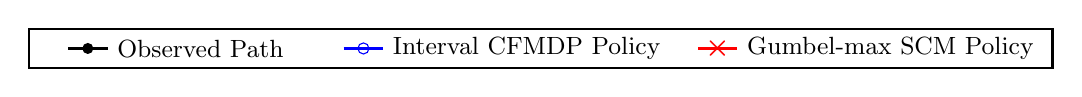
\begin{tikzpicture}[scale=1.0, every node/.style={scale=1.0}]
            \draw[thick, black] (-3, -0.25) rectangle (10, 0.25);
            %
            \draw[black, line width=1pt] (-2.5, 0.0) -- (-2,0.0);
            \fill[black] (-2.25,0.0) circle (2pt); %
            \node[right] at (-2,0.0) {\small Observed Path};
            
            %
            \draw[blue, line width=1pt] (1.0,0.0) -- (1.5,0.0);
            \node[draw=blue, circle, minimum size=4pt, inner sep=0pt] at (1.25,0.0) {}; %
            \node[right] at (1.5,0.0) {\small Interval CFMDP Policy};
            
            %
            \draw[red, line width=1pt] (5.5,0) -- (6,0);
            \node[red] at (5.75,0) {$\boldsymbol{\times}$}; %
            \node[right] at (6,0) {\small Gumbel-max SCM Policy};
        \end{tikzpicture}
    }\\
    %
    \subfigure[\footnotesize Lowest cumulative reward: Interval CFMDP ($312$), Gumbel-max SCM ($312$)]{%
        \resizebox{0.76\columnwidth}{!}{
             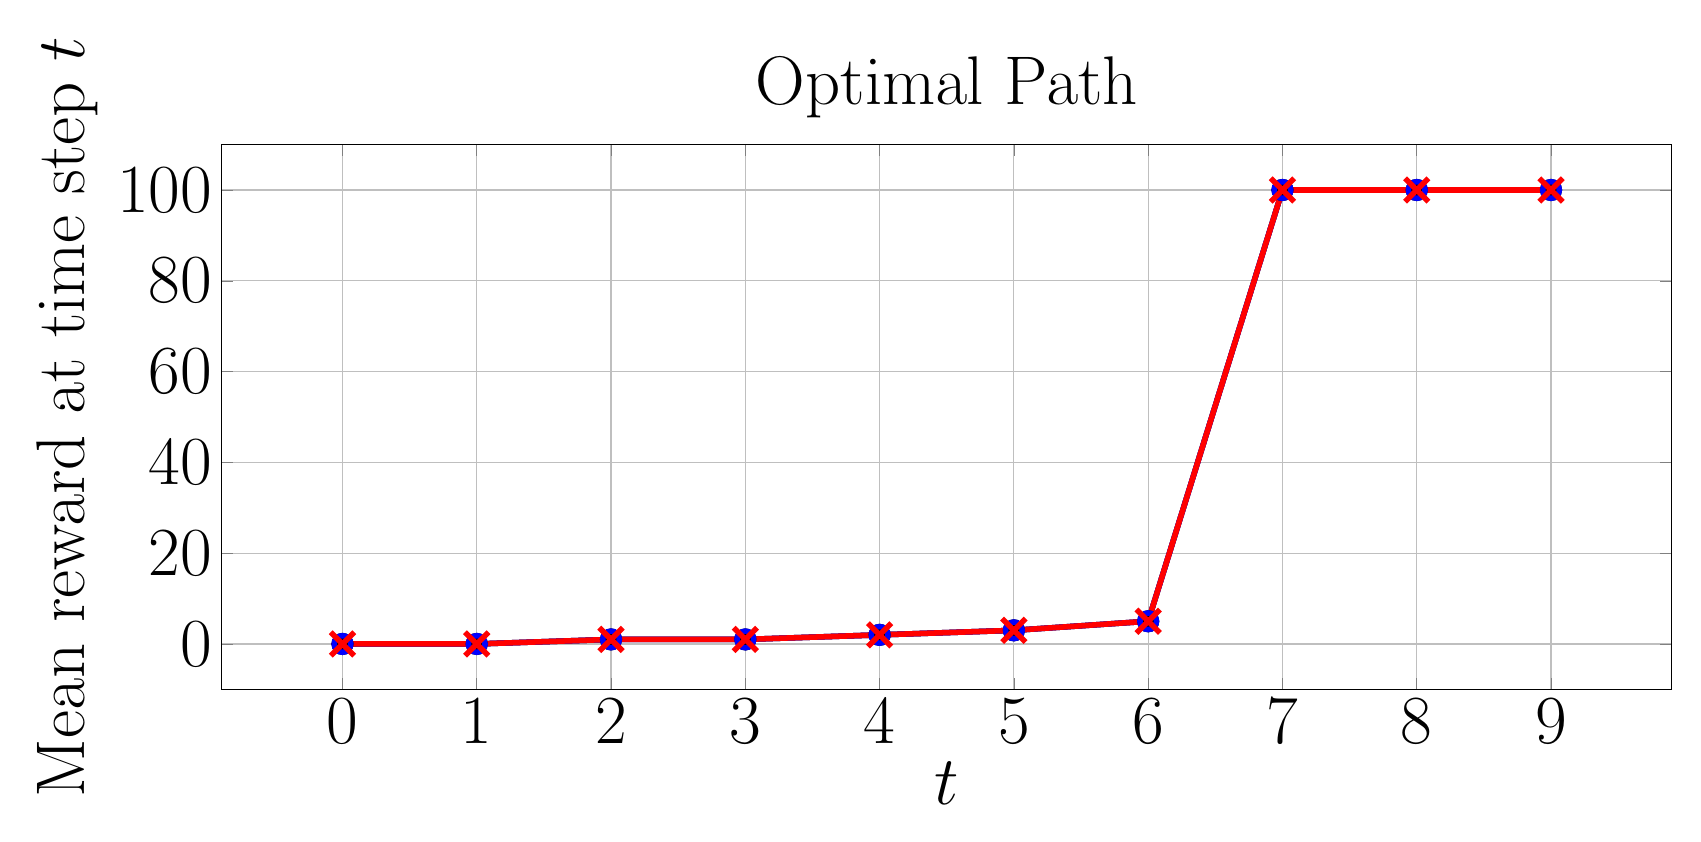
\begin{tikzpicture}
                \begin{axis}[
                    xlabel={$t$},
                    ylabel={Mean reward at time step $t$},
                    title={Optimal Path},
                    grid=both,
                    width=20cm, height=8.5cm,
                    every axis/.style={font=\Huge},
                    %
                ]
                \addplot[
                    color=black, %
                    mark=*, %
                    line width=2pt,
                    mark size=3pt,
                    error bars/.cd,
                    y dir=both, %
                    y explicit, %
                    error bar style={line width=1pt,solid},
                    error mark options={line width=1pt,mark size=4pt,rotate=90}
                ]
                coordinates {
                    (0, 0.0)  +- (0, 0.0)
                    (1, 0.0)  +- (0, 0.0) 
                    (2, 1.0)  +- (0, 0.0) 
                    (3, 1.0)  +- (0, 0.0)
                    (4, 2.0)  +- (0, 0.0)
                    (5, 3.0) +- (0, 0.0)
                    (6, 5.0) +- (0, 0.0)
                    (7, 100.0) +- (0, 0.0)
                    (8, 100.0) +- (0, 0.0)
                    (9, 100.0) +- (0, 0.0)
                };
                %
                \addplot[
                    color=blue, %
                    mark=o, %
                    line width=2pt,
                    mark size=3pt,
                    error bars/.cd,
                    y dir=both, %
                    y explicit, %
                    error bar style={line width=1pt,solid},
                    error mark options={line width=1pt,mark size=4pt,rotate=90}
                ]
                 coordinates {
                    (0, 0.0)  +- (0, 0.0)
                    (1, 0.0)  +- (0, 0.0) 
                    (2, 1.0)  +- (0, 0.0) 
                    (3, 1.0)  +- (0, 0.0)
                    (4, 2.0)  +- (0, 0.0)
                    (5, 3.0) +- (0, 0.0)
                    (6, 5.0) +- (0, 0.0)
                    (7, 100.0) +- (0, 0.0)
                    (8, 100.0) +- (0, 0.0)
                    (9, 100.0) +- (0, 0.0)
                };
                %
                \addplot[
                    color=red, %
                    mark=x, %
                    line width=2pt,
                    mark size=6pt,
                    error bars/.cd,
                    y dir=both, %
                    y explicit, %
                    error bar style={line width=1pt,solid},
                    error mark options={line width=1pt,mark size=4pt,rotate=90}
                ]
                coordinates {
                    (0, 0.0)  +- (0, 0.0)
                    (1, 0.0)  +- (0, 0.0) 
                    (2, 1.0)  +- (0, 0.0) 
                    (3, 1.0)  +- (0, 0.0)
                    (4, 2.0)  +- (0, 0.0)
                    (5, 3.0) +- (0, 0.0)
                    (6, 5.0) +- (0, 0.0)
                    (7, 100.0) +- (0, 0.0)
                    (8, 100.0) +- (0, 0.0)
                    (9, 100.0) +- (0, 0.0)
                };
                \end{axis}
            \end{tikzpicture}
         }
    }
    \hspace{1cm}
    \subfigure[\footnotesize Lowest cumulative reward: Interval CFMDP ($19$), Gumbel-max SCM ($-88$)]{%
         \resizebox{0.76\columnwidth}{!}{
            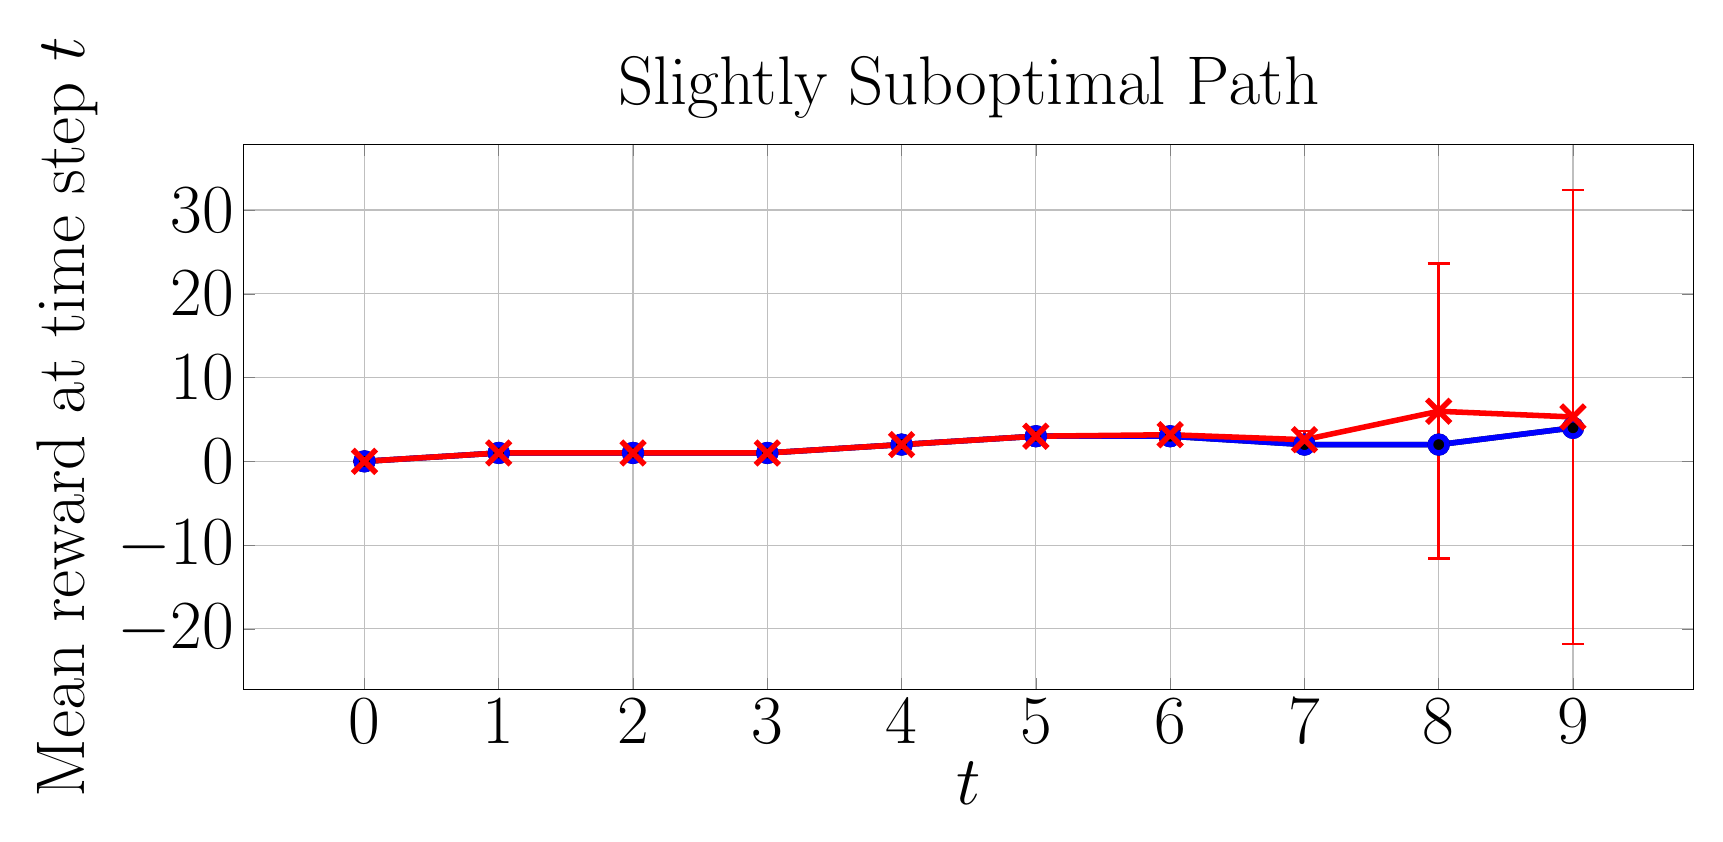
\begin{tikzpicture}
                \begin{axis}[
                    xlabel={$t$},
                    ylabel={Mean reward at time step $t$},
                    title={Slightly Suboptimal Path},
                    grid=both,
                    width=20cm, height=8.5cm,
                    every axis/.style={font=\Huge},
                    %
                ]
                \addplot[
                    color=black, %
                    mark=*, %
                    line width=2pt,
                    mark size=3pt,
                    error bars/.cd,
                    y dir=both, %
                    y explicit, %
                    error bar style={line width=1pt,solid},
                    error mark options={line width=1pt,mark size=4pt,rotate=90}
                ]
              coordinates {
                    (0, 0.0)  +- (0, 0.0)
                    (1, 1.0)  +- (0, 0.0) 
                    (2, 1.0)  +- (0, 0.0) 
                    (3, 1.0)  +- (0, 0.0)
                    (4, 2.0)  +- (0, 0.0)
                    (5, 3.0) +- (0, 0.0)
                    (6, 3.0) +- (0, 0.0)
                    (7, 2.0) +- (0, 0.0)
                    (8, 2.0) +- (0, 0.0)
                    (9, 4.0) +- (0, 0.0)
                };
                %
                \addplot[
                    color=blue, %
                    mark=o, %
                    line width=2pt,
                    mark size=3pt,
                    error bars/.cd,
                    y dir=both, %
                    y explicit, %
                    error bar style={line width=1pt,solid},
                    error mark options={line width=1pt,mark size=4pt,rotate=90}
                ]
              coordinates {
                    (0, 0.0)  +- (0, 0.0)
                    (1, 1.0)  +- (0, 0.0) 
                    (2, 1.0)  +- (0, 0.0) 
                    (3, 1.0)  +- (0, 0.0)
                    (4, 2.0)  +- (0, 0.0)
                    (5, 3.0) +- (0, 0.0)
                    (6, 3.0) +- (0, 0.0)
                    (7, 2.0) +- (0, 0.0)
                    (8, 2.0) +- (0, 0.0)
                    (9, 4.0) +- (0, 0.0)
                };
                %
                \addplot[
                    color=red, %
                    mark=x, %
                    line width=2pt,
                    mark size=6pt,
                    error bars/.cd,
                    y dir=both, %
                    y explicit, %
                    error bar style={line width=1pt,solid},
                    error mark options={line width=1pt,mark size=4pt,rotate=90}
                ]
                coordinates {
                    (0, 0.0)  +- (0, 0.0)
                    (1, 1.0)  +- (0, 0.0) 
                    (2, 1.0)  +- (0, 0.0) 
                    (3, 1.0)  +- (0, 0.0)
                    (4, 2.0)  += (0, 0.0)
                    (5, 3.0)  += (0, 0.0)
                    (6, 3.17847) += (0, 0.62606746) -= (0, 0.62606746)
                    (7, 2.5832885) += (0, 1.04598233) -= (0, 1.04598233)
                    (8, 5.978909) += (0, 17.60137623) -= (0, 17.60137623)
                    (9, 5.297059) += (0, 27.09227512) -= (0, 27.09227512)
                };
                \end{axis}
            \end{tikzpicture}
         }
    }\\[-1.5pt]
    \subfigure[\footnotesize Lowest cumulative reward: Interval CFMDP ($14$), Gumbel-max SCM ($-598$)]{%
         \resizebox{0.76\columnwidth}{!}{
             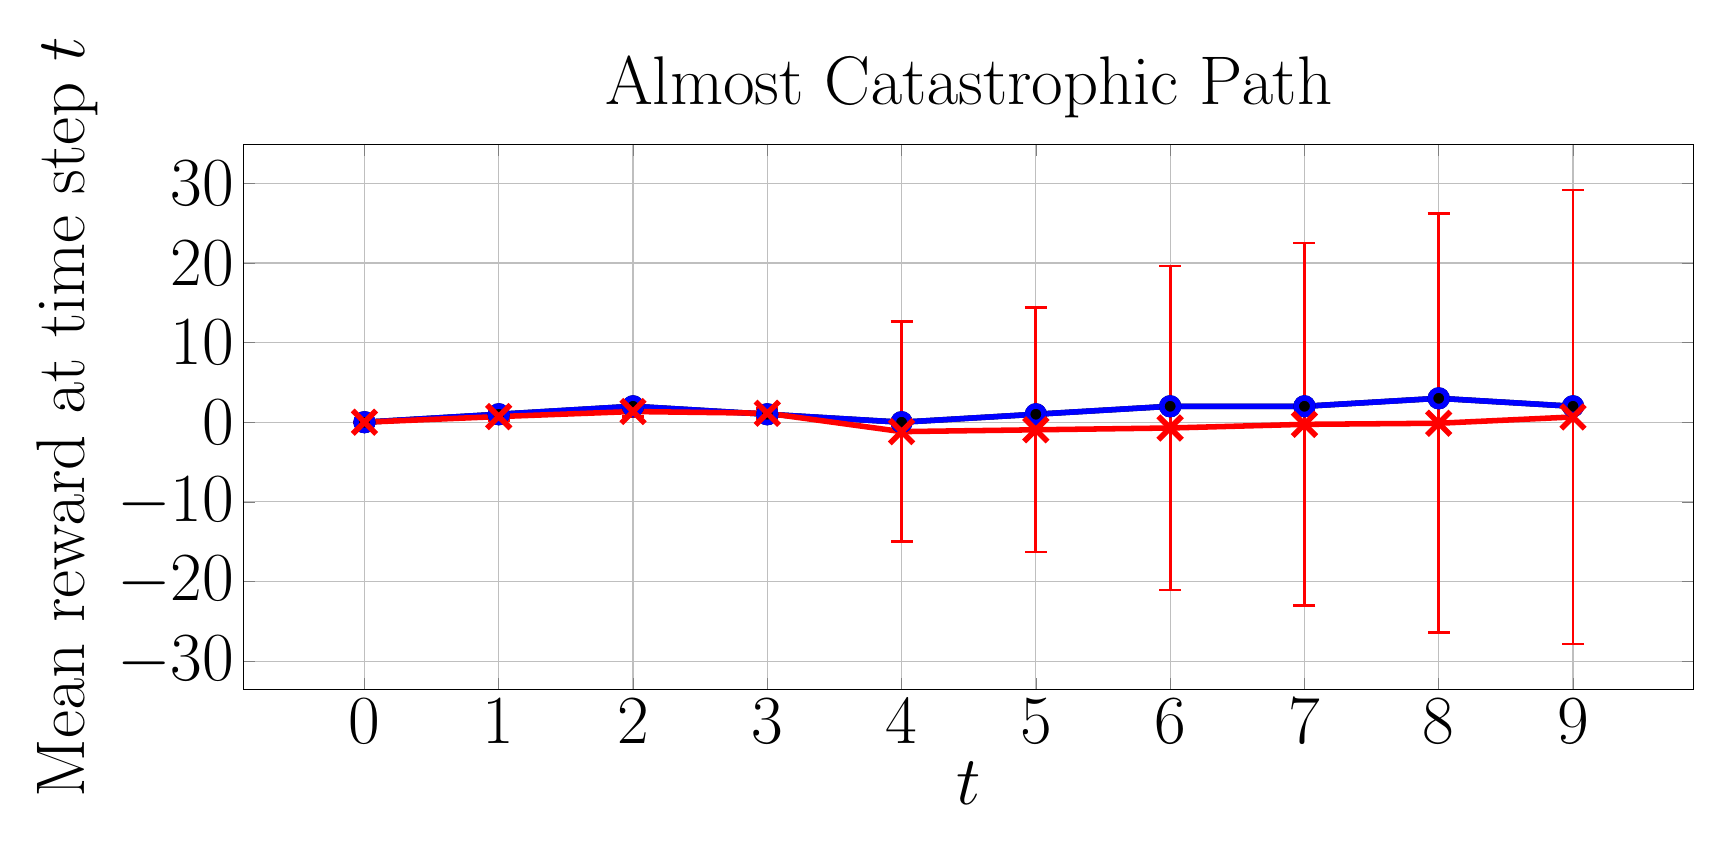
\begin{tikzpicture}
                \begin{axis}[
                    xlabel={$t$},
                    ylabel={Mean reward at time step $t$},
                    title={Almost Catastrophic Path},
                    grid=both,
                    width=20cm, height=8.5cm,
                    every axis/.style={font=\Huge},
                    %
                ]
                \addplot[
                    color=black, %
                    mark=*, %
                    line width=2pt,
                    mark size=3pt,
                    error bars/.cd,
                    y dir=both, %
                    y explicit, %
                    error bar style={line width=1pt,solid},
                    error mark options={line width=1pt,mark size=4pt,rotate=90}
                ]
                coordinates {
                    (0, 0.0)  +- (0, 0.0)
                    (1, 1.0)  +- (0, 0.0) 
                    (2, 2.0)  +- (0, 0.0) 
                    (3, 1.0)  +- (0, 0.0)
                    (4, 0.0)  +- (0, 0.0)
                    (5, 1.0) +- (0, 0.0)
                    (6, 2.0) +- (0, 0.0)
                    (7, 2.0) +- (0, 0.0)
                    (8, 3.0) +- (0, 0.0)
                    (9, 2.0) +- (0, 0.0)
                };
                %
                \addplot[
                    color=blue, %
                    mark=o, %
                    line width=2pt,
                    mark size=3pt,
                    error bars/.cd,
                    y dir=both, %
                    y explicit, %
                    error bar style={line width=1pt,solid},
                    error mark options={line width=1pt,mark size=4pt,rotate=90}
                ]
                coordinates {
                    (0, 0.0)  +- (0, 0.0)
                    (1, 1.0)  +- (0, 0.0) 
                    (2, 2.0)  +- (0, 0.0) 
                    (3, 1.0)  +- (0, 0.0)
                    (4, 0.0)  +- (0, 0.0)
                    (5, 1.0) +- (0, 0.0)
                    (6, 2.0) +- (0, 0.0)
                    (7, 2.0) +- (0, 0.0)
                    (8, 3.0) +- (0, 0.0)
                    (9, 2.0) +- (0, 0.0)
                };
                %
                \addplot[
                    color=red, %
                    mark=x, %
                    line width=2pt,
                    mark size=6pt,
                    error bars/.cd,
                    y dir=both, %
                    y explicit, %
                    error bar style={line width=1pt,solid},
                    error mark options={line width=1pt,mark size=4pt,rotate=90}
                ]
                coordinates {
                    (0, 0.0)  +- (0, 0.0)
                    (1, 0.7065655)  +- (0, 0.4553358) 
                    (2, 1.341673)  +- (0, 0.67091621) 
                    (3, 1.122926)  +- (0, 0.61281824)
                    (4, -1.1821935)  +- (0, 13.82444042)
                    (5, -0.952399)  +- (0, 15.35195457)
                    (6, -0.72672) +- (0, 20.33508414)
                    (7, -0.268983) +- (0, 22.77861454)
                    (8, -0.1310835) +- (0, 26.31013314)
                    (9, 0.65806) +- (0, 28.50670214)
                };
                %
            %
            %
            %
            %
            %
            %
            %
            %
            %
            %
            %
            %
            %
            %
            %
            %
            %
            %
                \end{axis}
            \end{tikzpicture}
         }
    }
    \hspace{1cm}
    \subfigure[\footnotesize Lowest cumulative reward: Interval CFMDP ($-698$), Gumbel-max SCM ($-698$)]{%
         \resizebox{0.76\columnwidth}{!}{
            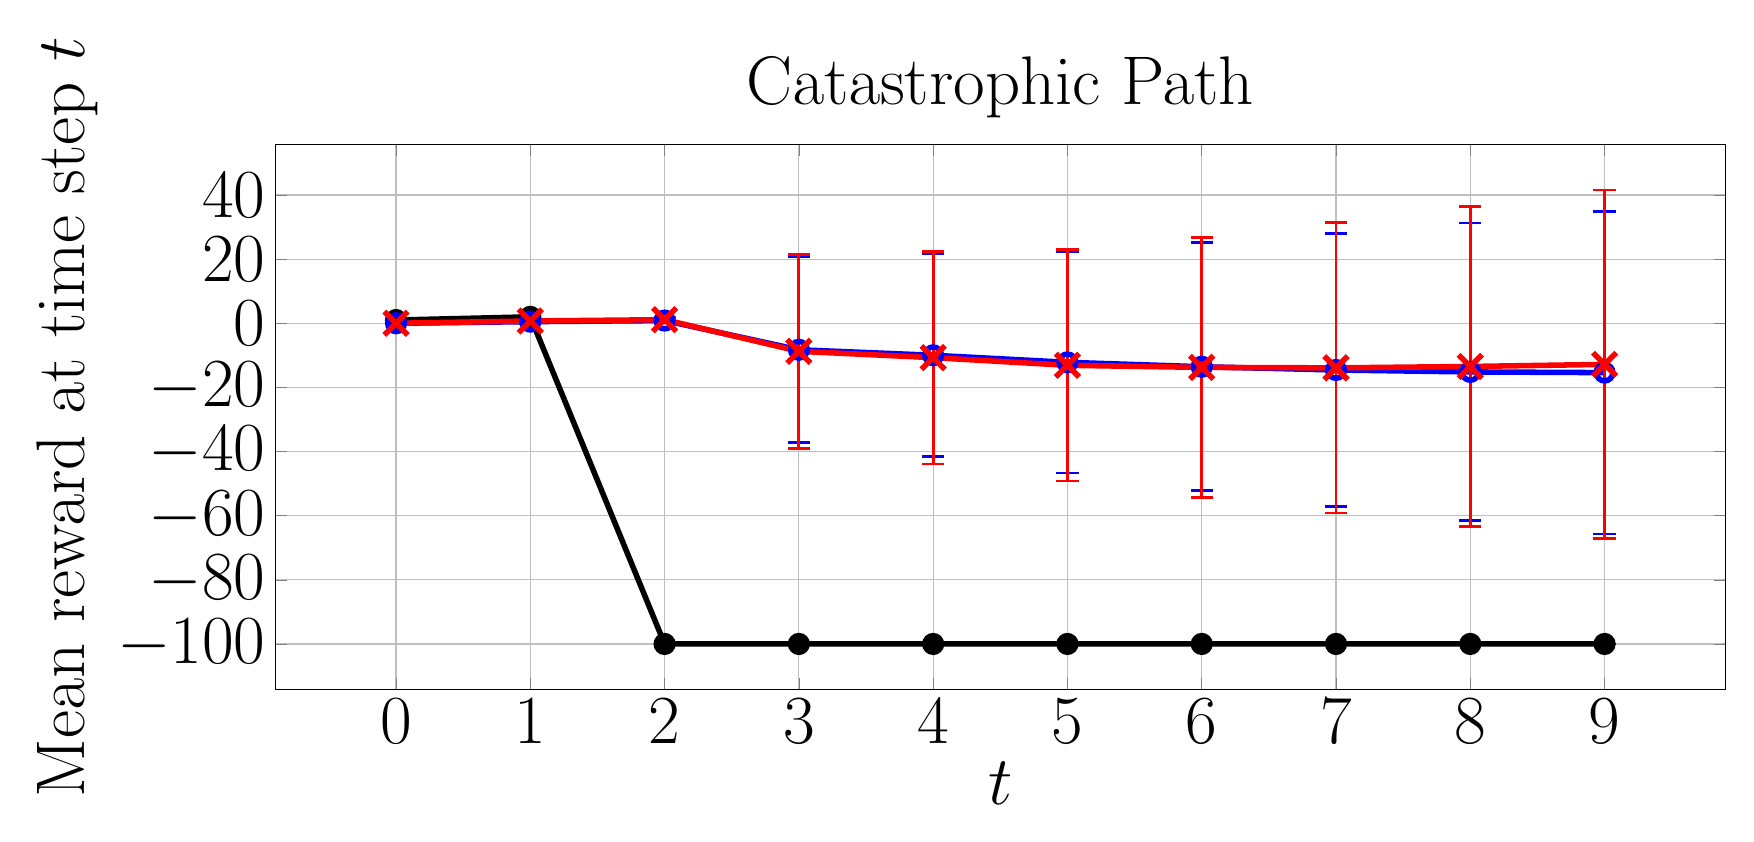
\begin{tikzpicture}
                \begin{axis}[
                    xlabel={$t$},
                    ylabel={Mean reward at time step $t$},
                    title={Catastrophic Path},
                    grid=both,
                    width=20cm, height=8.5cm,
                    every axis/.style={font=\Huge},
                    %
                ]
                \addplot[
                    color=black, %
                    mark=*, %
                    line width=2pt,
                    mark size=3pt,
                    error bars/.cd,
                    y dir=both, %
                    y explicit, %
                    error bar style={line width=1pt,solid},
                    error mark options={line width=1pt,mark size=4pt,rotate=90}
                ]
                coordinates {
                    (0, 1.0)  +- (0, 0.0)
                    (1, 2.0)  +- (0, 0.0) 
                    (2, -100.0)  +- (0, 0.0) 
                    (3, -100.0)  +- (0, 0.0)
                    (4, -100.0)  +- (0, 0.0)
                    (5, -100.0) +- (0, 0.0)
                    (6, -100.0) +- (0, 0.0)
                    (7, -100.0) +- (0, 0.0)
                    (8, -100.0) +- (0, 0.0)
                    (9, -100.0) +- (0, 0.0)
                };
                %
                \addplot[
                    color=blue, %
                    mark=o, %
                    line width=2pt,
                    mark size=3pt,
                    error bars/.cd,
                    y dir=both, %
                    y explicit, %
                    error bar style={line width=1pt,solid},
                    error mark options={line width=1pt,mark size=4pt,rotate=90}
                ]
                coordinates {
                    (0, 0.0)  +- (0, 0.0)
                    (1, 0.504814)  +- (0, 0.49997682) 
                    (2, 0.8439835)  +- (0, 0.76831917) 
                    (3, -8.2709165)  +- (0, 28.93656754)
                    (4, -9.981082)  +- (0, 31.66825363)
                    (5, -12.1776325) +- (0, 34.53463233)
                    (6, -13.556076) +- (0, 38.62845372)
                    (7, -14.574418) +- (0, 42.49603359)
                    (8, -15.1757075) +- (0, 46.41913968)
                    (9, -15.3900395) +- (0, 50.33563368)
                };
                %
                \addplot[
                    color=red, %
                    mark=x, %
                    line width=2pt,
                    mark size=6pt,
                    error bars/.cd,
                    y dir=both, %
                    y explicit, %
                    error bar style={line width=1pt,solid},
                    error mark options={line width=1pt,mark size=4pt,rotate=90}
                ]
                coordinates {
                    (0, 0.0)  +- (0, 0.0)
                    (1, 0.701873)  +- (0, 0.45743556) 
                    (2, 1.1227805)  +- (0, 0.73433129) 
                    (3, -8.7503255)  +- (0, 30.30257976)
                    (4, -10.722092)  +- (0, 33.17618589)
                    (5, -13.10721)  +- (0, 36.0648089)
                    (6, -13.7631645) +- (0, 40.56553451)
                    (7, -13.909043) +- (0, 45.23829402)
                    (8, -13.472517) +- (0, 49.96270296)
                    (9, -12.8278835) +- (0, 54.38618735)
                };
                %
            %
            %
            %
            %
            %
            %
            %
            %
            %
            %
            %
            %
            %
            %
            %
            %
            %
            %
                \end{axis}
            \end{tikzpicture}
         }
    }
    \caption{Average instant reward of CF paths induced by policies on GridWorld $p=0.4$.}
    \label{fig: reward p=0.4}
\end{figure*}

\subsection{Experimental Setup}
To compare policy performance, we measure the average rewards of counterfactual paths induced by our policy and the Gumbel-max policy by uniformly sampling $200$ counterfactual MDPs from the ICFMDP and generating $10,000$ counterfactual paths over each sampled CFMDP. \jl{Since the interval CFMDP depends on the observed path, we select $4$  paths of varying optimality to evaluate how the observed path impacts the performance of both policies: an optimal path, a slightly suboptimal path that could reach the optimal reward with a few changes, a catastrophic path that enters a catastrophic, terminal state with low reward, and an almost catastrophic path that was close to entering a catastrophic state.} When measuring the average probability bound widths and execution time needed to generate the ICFMDPs, we averaged over $20$ randomly generated observed paths
\footnote{Further training details are provided in Appendix \ref{app: training details}, and the code is provided at \href{https://github.com/ddv-lab/robust-cf-inference-in-MDPs}{https://github.com/ddv-lab/robust-cf-inference-in-MDPs}
%
%
.}.

\subsection{GridWorld}
\jl{The GridWorld MDP is a $4 \times 4$ grid where an agent must navigate from the top-left corner to the goal state in the bottom-right corner, avoiding a dangerous terminal state in the centre. At each time step, the agent can move up, down, left, or right, but there is a small probability (controlled by hyper-parameter $p$) of moving in an unintended direction. As the agent nears the goal, the reward for each state increases, culminating in a reward of $+100$ for reaching the goal. Entering the dangerous state results in a penalty of $-100$. We use two versions of GridWorld: a less stochastic version with $p=0.9$ (i.e., $90$\% chance of moving in the chosen direction) and a more stochastic version with $p=0.4$.}

\paragraph{GridWorld ($p=0.9$)}
When $p=0.9$, the counterfactual probability bounds are typically narrow (see Table \ref{tab:nonzero_probs} for average measurements). Consequently, as shown in Figure \ref{fig: reward p=0.9}, both policies are nearly identical and perform similarly well across the optimal, slightly suboptimal, and catastrophic paths.
%
However, for the almost catastrophic path, the interval CFMDP path is more conservative and follows the observed path more closely (as this is where the probability bounds are narrowest), which typically requires one additional step to reach the goal state than the Gumbel-max SCM policy.
%

\paragraph{GridWorld ($p=0.4$)}
\jl{When $p=0.4$, the GridWorld environment becomes more uncertain, increasing the risk of entering the dangerous state even if correct actions are chosen. Thus, as shown in Figure \ref{fig: reward p=0.4}, the interval CFMDP policy adopts a more conservative approach, avoiding deviation from the observed policy if it cannot guarantee higher counterfactual rewards (see the slightly suboptimal and almost catastrophic paths), whereas the Gumbel-max SCM is inconsistent: it can yield higher rewards, but also much lower rewards, reflected in the wide error bars.} For the catastrophic path, both policies must deviate from the observed path to achieve a higher reward and, in this case, perform similarly.
%
%
%
%
\subsection{Sepsis}
The Sepsis MDP \citep{oberst2019counterfactual} simulates trajectories of Sepsis patients. Each state consists of four vital signs (heart rate, blood pressure, oxygen concentration, and glucose levels), categorised as low, normal, or high.
and three treatments that can be toggled on/off at each time step (8 actions in total). Unlike \citet{oberst2019counterfactual}, we scale rewards based on the number of out-of-range vital signs, between $-1000$ (patient dies) and $1000$ (patient discharged). \jl{Like the GridWorld $p=0.4$ experiment, the Sepsis MDP is highly uncertain, as many states are equally likely to lead to optimal and poor outcomes. Thus, as shown in Figure \ref{fig: reward sepsis}, both policies follow the observed optimal and almost catastrophic paths to guarantee rewards are no worse than the observation.} However, improving the catastrophic path requires deviating from the observation. Here, the Gumbel-max SCM policy, on average, performs better than the interval CFMDP policy. But, since both policies have lower bounds clipped at $-1000$, neither policy reliably improves over the observation. In contrast, for the slightly suboptimal path, the interval CFMDP policy performs significantly better, shown by its higher lower bounds. 
Moreover, in these two cases, the worst-case counterfactual path generated by the interval CFMDP policy is better than that of the Gumbel-max SCM policy,
indicating its greater robustness.
%
\begin{figure*}
    \centering
     \resizebox{0.6\textwidth}{!}{
        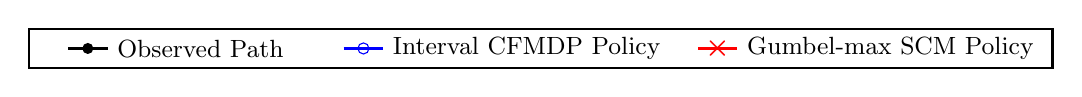
\begin{tikzpicture}[scale=1.0, every node/.style={scale=1.0}]
            \draw[thick, black] (-3, -0.25) rectangle (10, 0.25);
            %
            \draw[black, line width=1pt] (-2.5, 0.0) -- (-2,0.0);
            \fill[black] (-2.25,0.0) circle (2pt); %
            \node[right] at (-2,0.0) {\small Observed Path};
            
            %
            \draw[blue, line width=1pt] (1.0,0.0) -- (1.5,0.0);
            \node[draw=blue, circle, minimum size=4pt, inner sep=0pt] at (1.25,0.0) {}; %
            \node[right] at (1.5,0.0) {\small Interval CFMDP Policy};
            
            %
            \draw[red, line width=1pt] (5.5,0) -- (6,0);
            \node[red] at (5.75,0) {$\boldsymbol{\times}$}; %
            \node[right] at (6,0) {\small Gumbel-max SCM Policy};
        \end{tikzpicture}
    }\\
    \subfigure[\footnotesize Lowest cumulative reward: Interval CFMDP ($8000$), Gumbel-max SCM ($8000$)]{%
         \resizebox{0.76\columnwidth}{!}{
             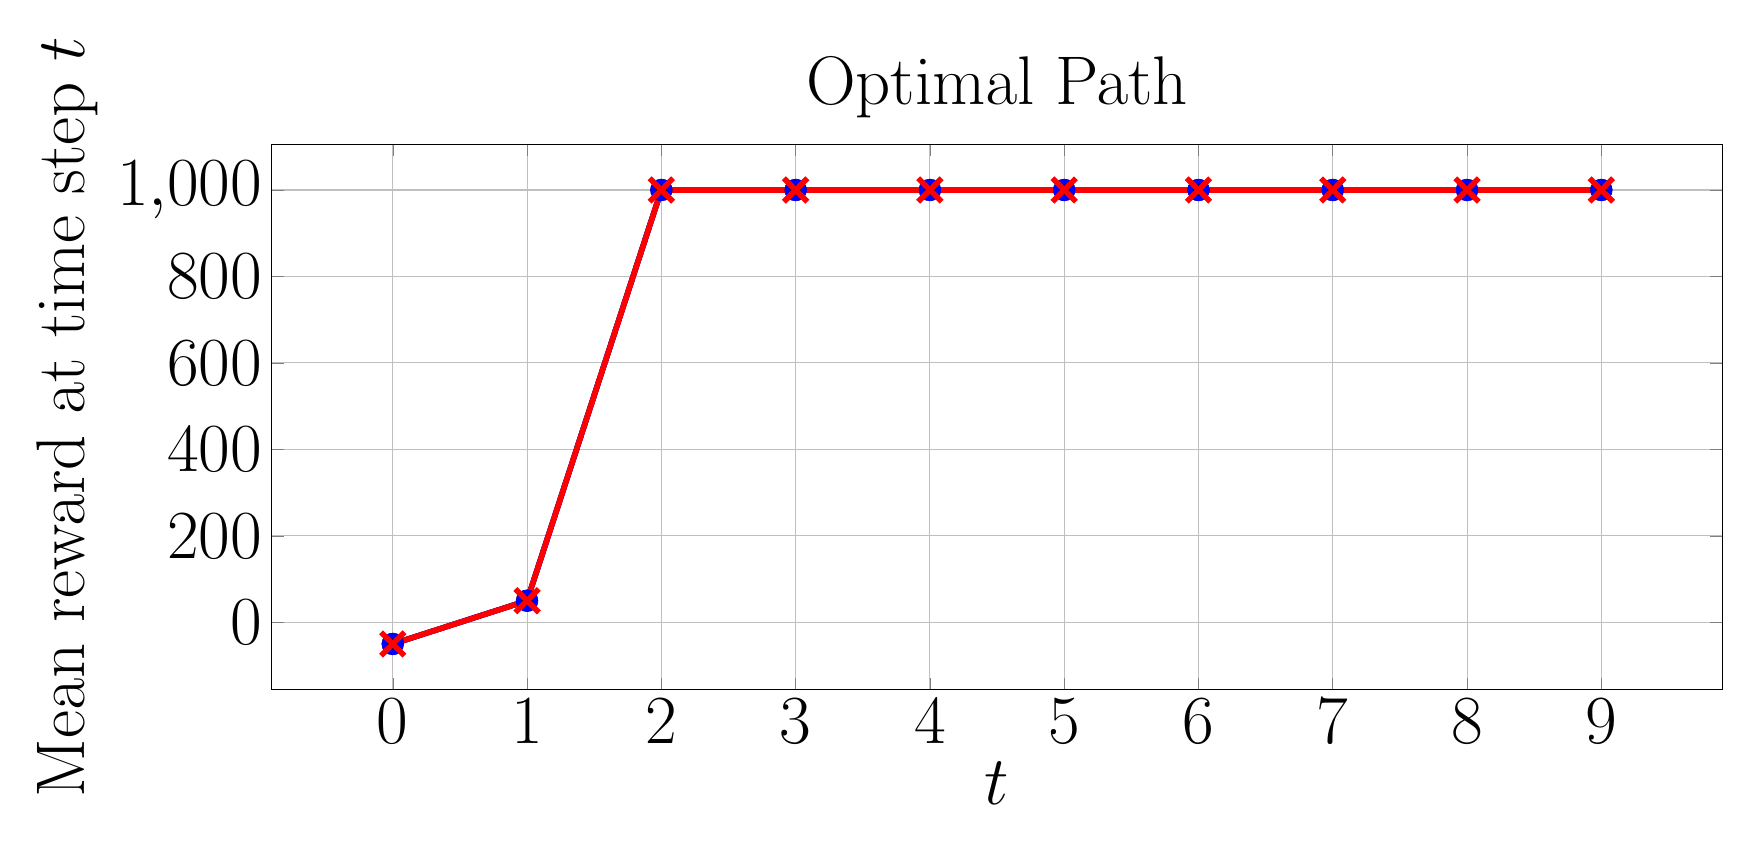
\begin{tikzpicture}
                \begin{axis}[
                    xlabel={$t$},
                    ylabel={Mean reward at time step $t$},
                    title={Optimal Path},
                    grid=both,
                    width=20cm, height=8.5cm,
                    every axis/.style={font=\Huge},
                    %
                ]
                \addplot[
                    color=black, %
                    mark=*, %
                    line width=2pt,
                    mark size=3pt,
                ]
                coordinates {
                    (0, -50.0)
                    (1, 50.0)
                    (2, 1000.0)
                    (3, 1000.0)
                    (4, 1000.0)
                    (5, 1000.0)
                    (6, 1000.0)
                    (7, 1000.0)
                    (8, 1000.0)
                    (9, 1000.0)
                };
                %
                \addplot[
                    color=blue, %
                    mark=o, %
                    line width=2pt,
                    mark size=3pt,
                    error bars/.cd,
                    y dir=both, %
                    y explicit, %
                    error bar style={line width=1pt,solid},
                    error mark options={line width=1pt,mark size=4pt,rotate=90}
                ]
                coordinates {
                    (0, -50.0)  +- (0, 0.0)
                    (1, 50.0)  +- (0, 0.0) 
                    (2, 1000.0)  +- (0, 0.0) 
                    (3, 1000.0)  +- (0, 0.0)
                    (4, 1000.0)  +- (0, 0.0)
                    (5, 1000.0) +- (0, 0.0)
                    (6, 1000.0) +- (0, 0.0)
                    (7, 1000.0) +- (0, 0.0)
                    (8, 1000.0) +- (0, 0.0)
                    (9, 1000.0) +- (0, 0.0)
                };
                %
                \addplot[
                    color=red, %
                    mark=x, %
                    line width=2pt,
                    mark size=6pt,
                    error bars/.cd,
                    y dir=both, %
                    y explicit, %
                    error bar style={line width=1pt,solid},
                    error mark options={line width=1pt,mark size=4pt,rotate=90}
                ]
                coordinates {
                    (0, -50.0)  +- (0, 0.0)
                    (1, 50.0)  +- (0, 0.0) 
                    (2, 1000.0)  +- (0, 0.0) 
                    (3, 1000.0)  +- (0, 0.0)
                    (4, 1000.0)  +- (0, 0.0)
                    (5, 1000.0) +- (0, 0.0)
                    (6, 1000.0) +- (0, 0.0)
                    (7, 1000.0) +- (0, 0.0)
                    (8, 1000.0) +- (0, 0.0)
                    (9, 1000.0) +- (0, 0.0)
                };
                %
                \end{axis}
            \end{tikzpicture}
         }
    }
    \hspace{1cm}
    \subfigure[\footnotesize Lowest cumulative reward: Interval CFMDP ($-5980$), Gumbel-max SCM ($-8000$)]{%
         \resizebox{0.76\columnwidth}{!}{
            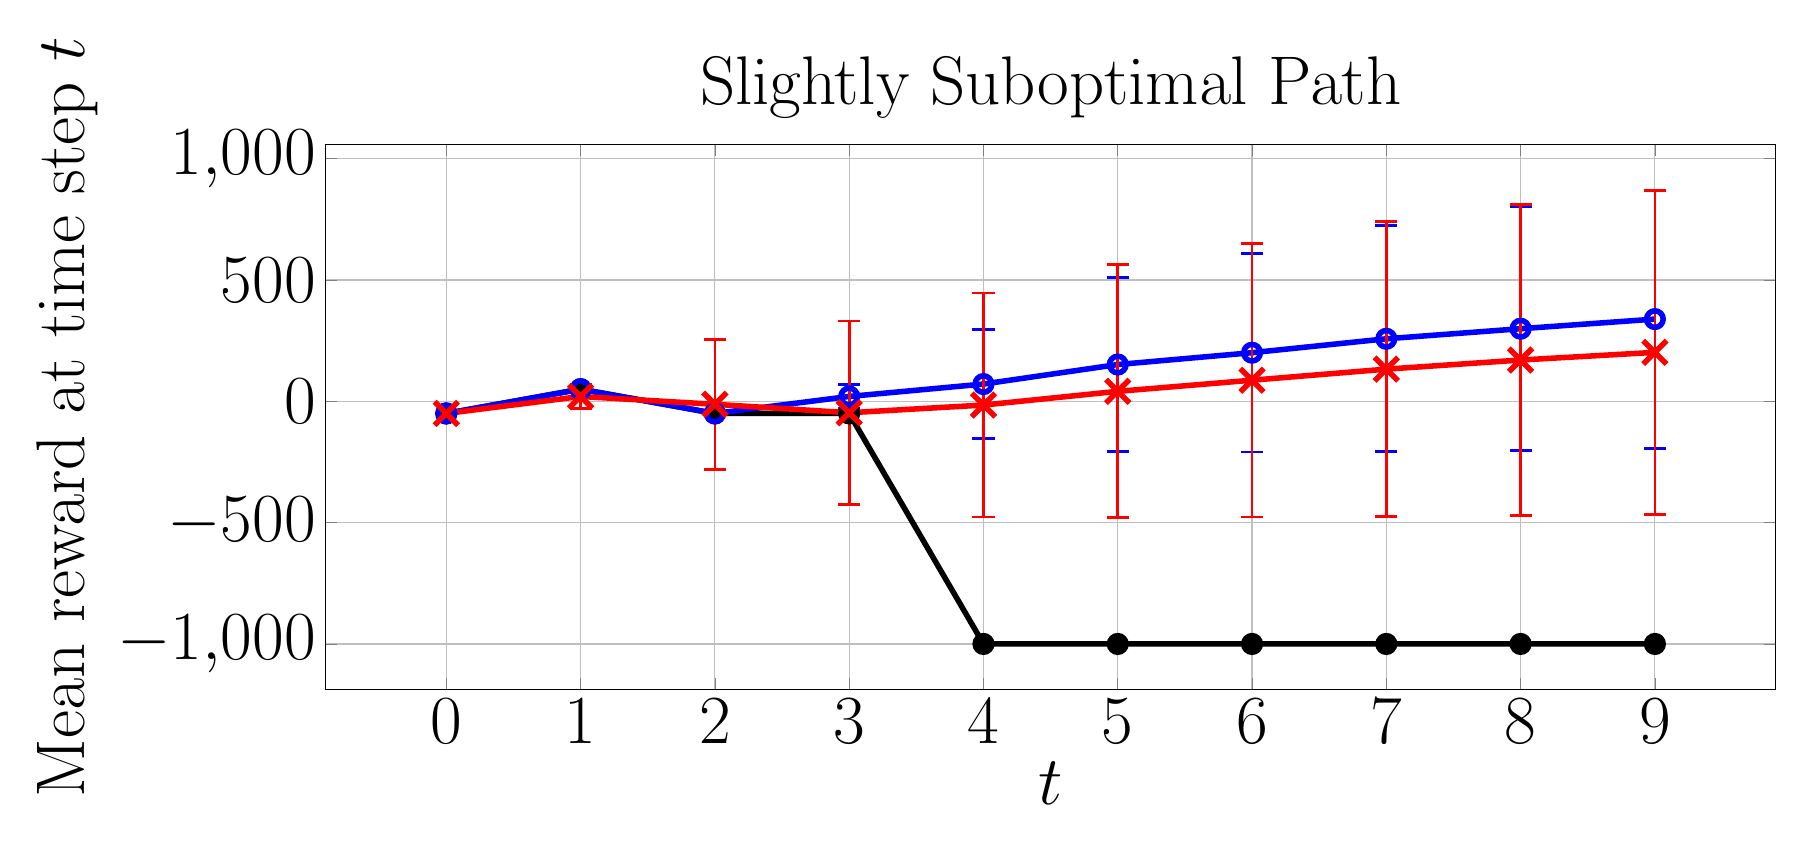
\begin{tikzpicture}
                \begin{axis}[
                    xlabel={$t$},
                    ylabel={Mean reward at time step $t$},
                    title={Slightly Suboptimal Path},
                    grid=both,
                    width=20cm, height=8.5cm,
                    every axis/.style={font=\Huge},
                    %
                ]
               \addplot[
                    color=black, %
                    mark=*, %
                    line width=2pt,
                    mark size=3pt,
                ]
                coordinates {
                    (0, -50.0)
                    (1, 50.0)
                    (2, -50.0)
                    (3, -50.0)
                    (4, -1000.0)
                    (5, -1000.0)
                    (6, -1000.0)
                    (7, -1000.0)
                    (8, -1000.0)
                    (9, -1000.0)
                };
                %
                \addplot[
                    color=blue, %
                    mark=o, %
                    line width=2pt,
                    mark size=3pt,
                    error bars/.cd,
                    y dir=both, %
                    y explicit, %
                    error bar style={line width=1pt,solid},
                    error mark options={line width=1pt,mark size=4pt,rotate=90}
                ]
                coordinates {
                    (0, -50.0)  +- (0, 0.0)
                    (1, 50.0)  +- (0, 0.0) 
                    (2, -50.0)  +- (0, 0.0) 
                    (3, 20.0631)  +- (0, 49.97539413)
                    (4, 71.206585)  +- (0, 226.02033693)
                    (5, 151.60797) +- (0, 359.23292559)
                    (6, 200.40593) +- (0, 408.86185176)
                    (7, 257.77948) +- (0, 466.10372804)
                    (8, 299.237465) +- (0, 501.82579506)
                    (9, 338.9129) +- (0, 532.06124996)
                };
                %
                \addplot[
                    color=red, %
                    mark=x, %
                    line width=2pt,
                    mark size=6pt,
                    error bars/.cd,
                    y dir=both, %
                    y explicit, %
                    error bar style={line width=1pt,solid},
                    error mark options={line width=1pt,mark size=4pt,rotate=90}
                ]
                coordinates {
                    (0, -50.0)  +- (0, 0.0)
                    (1, 20.00736)  +- (0, 49.99786741) 
                    (2, -12.282865)  +- (0, 267.598755) 
                    (3, -47.125995)  +- (0, 378.41755832)
                    (4, -15.381965)  +- (0, 461.77616558)
                    (5, 41.15459) +- (0, 521.53189262)
                    (6, 87.01595) +- (0, 564.22243126 )
                    (7, 132.62376) +- (0, 607.31338037)
                    (8, 170.168145) +- (0, 641.48013693)
                    (9, 201.813135) +- (0, 667.29441777)
                };
                %
                %
                %
                %
                %
                %
                %
                %
                %
                %
                %
                %
                %
                %
                %
                %
                %
                %
                %
                \end{axis}
            \end{tikzpicture}
         }
    }\\[-1.5pt]
    \subfigure[\footnotesize Lowest cumulative reward: Interval CFMDP ($100$), Gumbel-max SCM ($100$)]{%
         \resizebox{0.76\columnwidth}{!}{
             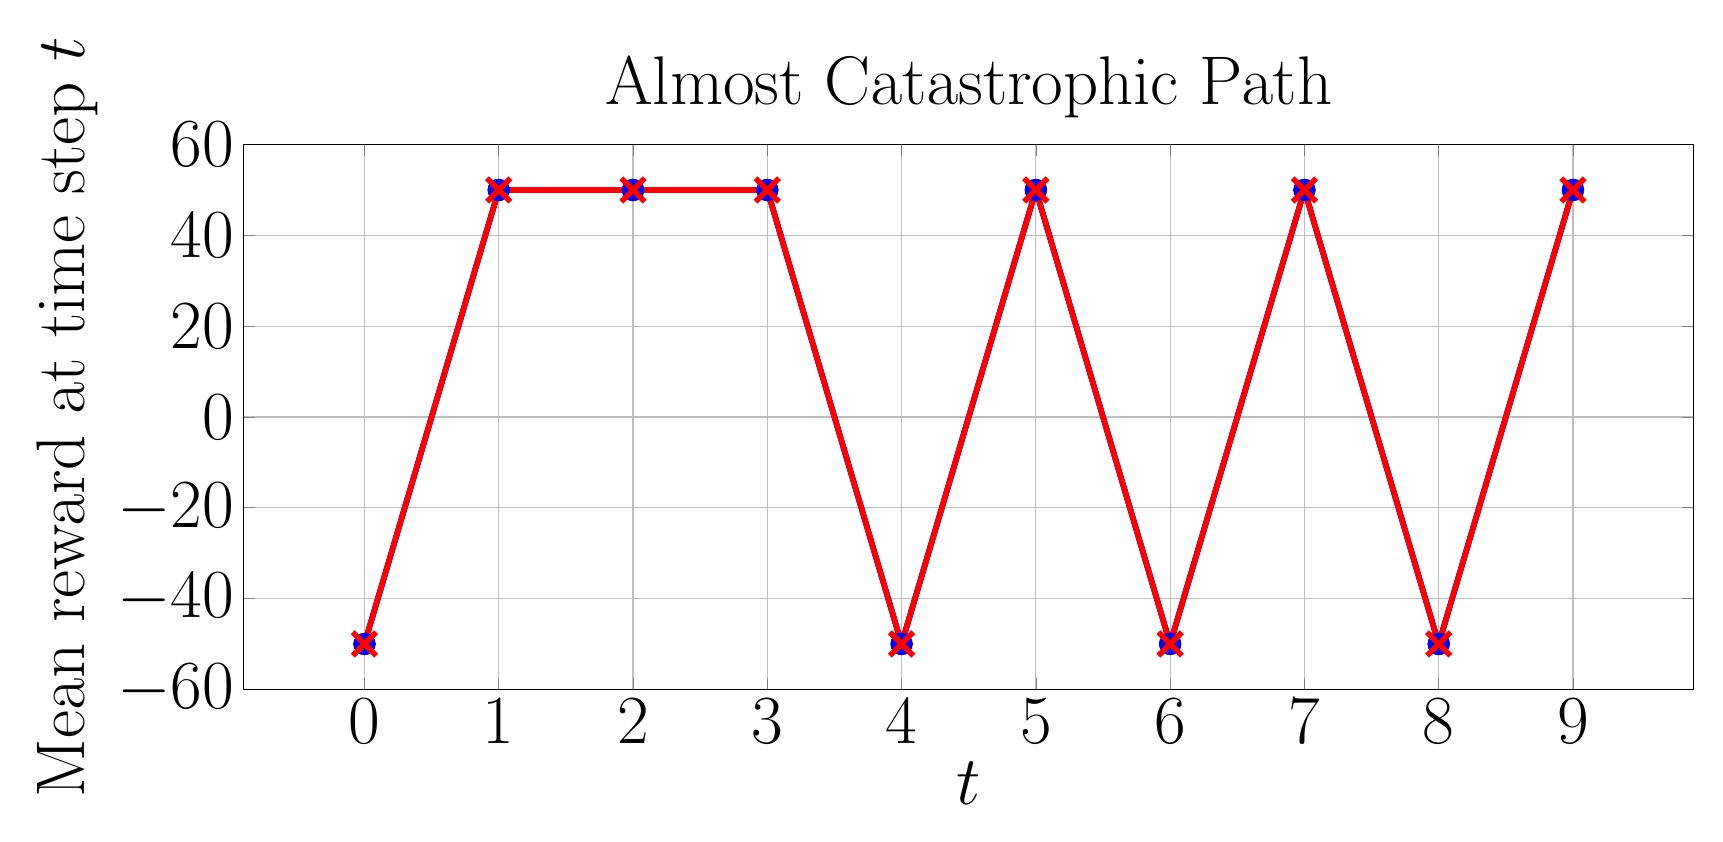
\begin{tikzpicture}
                \begin{axis}[
                    xlabel={$t$},
                    ylabel={Mean reward at time step $t$},
                    title={Almost Catastrophic Path},
                    grid=both,
                    every axis/.style={font=\Huge},
                    width=20cm, height=8.5cm,
                    %
                ]
               \addplot[
                    color=black, %
                    mark=*, %
                    line width=2pt,
                    mark size=3pt,
                ]
                coordinates {
                    (0, -50.0)
                    (1, 50.0)
                    (2, 50.0)
                    (3, 50.0)
                    (4, -50.0)
                    (5, 50.0)
                    (6, -50.0)
                    (7, 50.0)
                    (8, -50.0)
                    (9, 50.0)
                };
                %
                %
                \addplot[
                    color=blue, %
                    mark=o, %
                    line width=2pt,
                    mark size=3pt,
                    error bars/.cd,
                    y dir=both, %
                    y explicit, %
                    error bar style={line width=1pt,solid},
                    error mark options={line width=1pt,mark size=4pt,rotate=90}
                ]
                coordinates {
                    (0, -50.0)  +- (0, 0.0)
                    (1, 50.0)  +- (0, 0.0) 
                    (2, 50.0)  +- (0, 0.0) 
                    (3, 50.0)  +- (0, 0.0)
                    (4, -50.0)  +- (0, 0.0)
                    (5, 50.0) +- (0, 0.0)
                    (6, -50.0) +- (0, 0.0)
                    (7, 50.0) +- (0, 0.0)
                    (8, -50.0) +- (0, 0.0)
                    (9, 50.0) +- (0, 0.0)
                };
                %
                \addplot[
                    color=red, %
                    mark=x, %
                    line width=2pt,
                    mark size=6pt,
                    error bars/.cd,
                    y dir=both, %
                    y explicit, %
                    error bar style={line width=1pt,solid},
                    error mark options={line width=1pt,mark size=4pt,rotate=90}
                ]
                coordinates {
                    (0, -50.0)  +- (0, 0.0)
                    (1, 50.0)  +- (0, 0.0) 
                    (2, 50.0)  +- (0, 0.0) 
                    (3, 50.0)  +- (0, 0.0)
                    (4, -50.0)  +- (0, 0.0)
                    (5, 50.0) +- (0, 0.0)
                    (6, -50.0) +- (0, 0.0)
                    (7, 50.0) +- (0, 0.0)
                    (8, -50.0) +- (0, 0.0)
                    (9, 50.0) +- (0, 0.0)
                };
                %
                %
                %
                %
                %
                %
                %
                %
                %
                %
                %
                %
                %
                %
                %
                %
                %
                %
                %
                \end{axis}
            \end{tikzpicture}
         }
    }
    \hspace{1cm}
    \subfigure[\footnotesize Lowest cumulative reward: Interval CFMDP ($-7150$), Gumbel-max SCM ($-9050$)]{%
         \resizebox{0.76\columnwidth}{!}{
            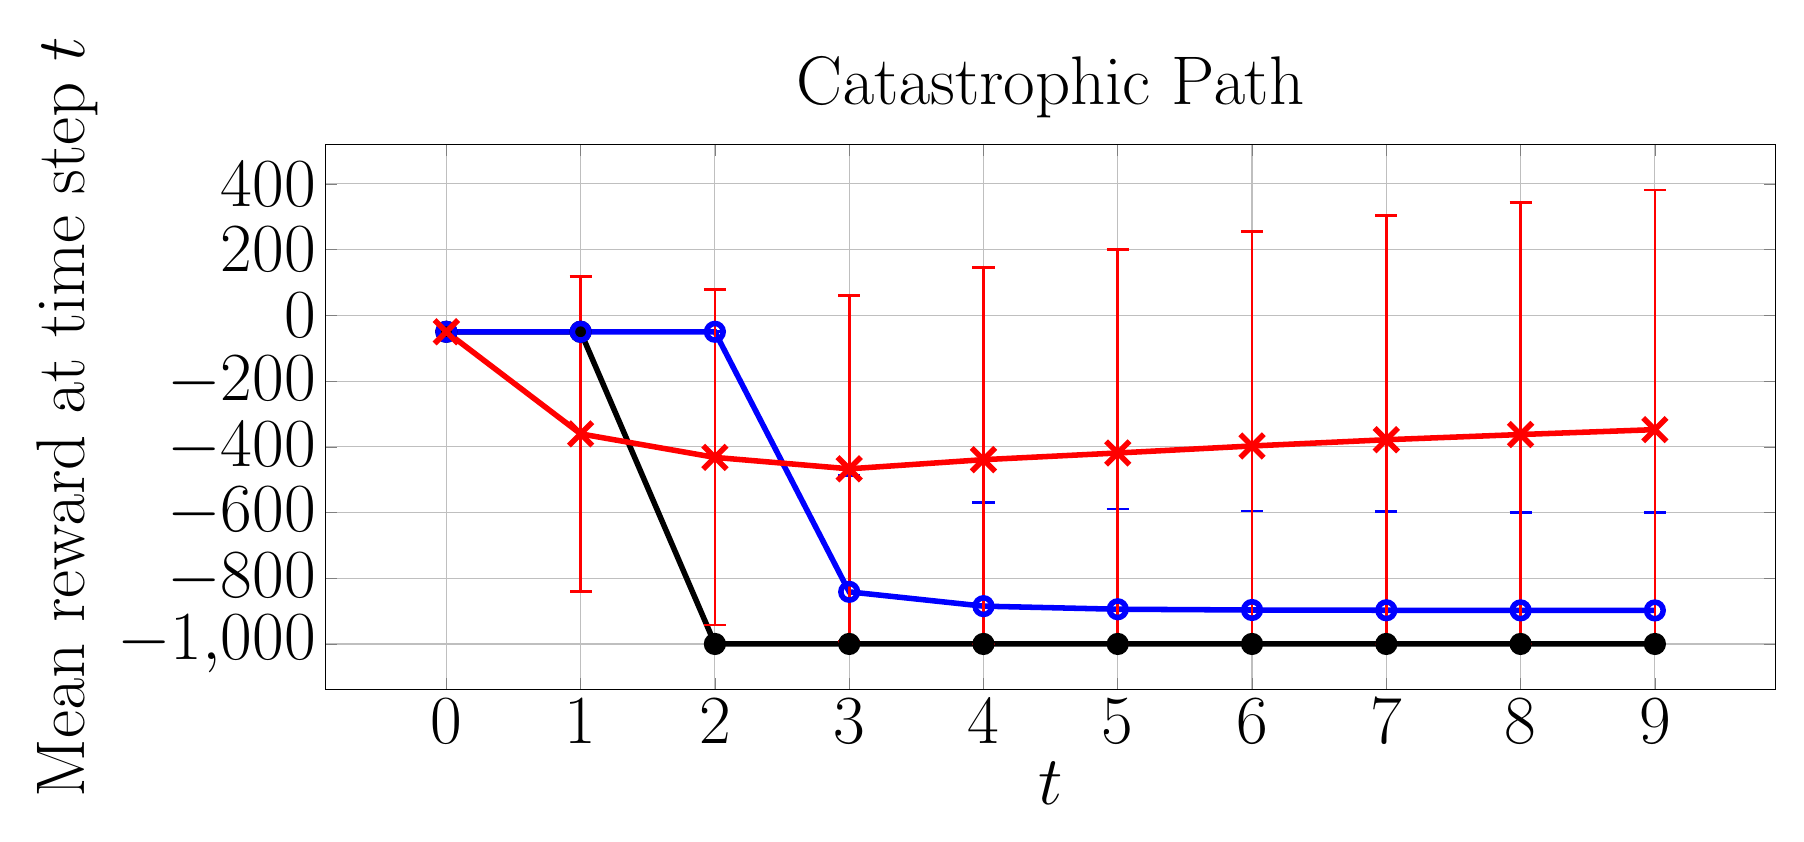
\begin{tikzpicture}
                \begin{axis}[
                    xlabel={$t$},
                    ylabel={Mean reward at time step $t$},
                    title={Catastrophic Path},
                    grid=both,
                    width=20cm, height=8.5cm,
                    every axis/.style={font=\Huge},
                    %
                ]
               \addplot[
                    color=black, %
                    mark=*, %
                    line width=2pt,
                    mark size=3pt,
                ]
                coordinates {
                    (0, -50.0)
                    (1, -50.0)
                    (2, -1000.0)
                    (3, -1000.0)
                    (4, -1000.0)
                    (5, -1000.0)
                    (6, -1000.0)
                    (7, -1000.0)
                    (8, -1000.0)
                    (9, -1000.0)
                };
                %
                %
                \addplot[
                    color=blue, %
                    mark=o, %
                    line width=2pt,
                    mark size=3pt,
                    error bars/.cd,
                    y dir=both, %
                    y explicit, %
                    error bar style={line width=1pt,solid},
                    error mark options={line width=1pt,mark size=4pt,rotate=90}
                ]
                coordinates {
                    (0, -50.0)  +- (0, 0.0)
                    (1, -50.0)  +- (0, 0.0) 
                    (2, -50.0)  +- (0, 0.0) 
                    (3, -841.440725)  += (0, 354.24605512) -= (0, 158.559275)
                    (4, -884.98225)  += (0, 315.37519669) -= (0, 115.01775)
                    (5, -894.330425) += (0, 304.88572805) -= (0, 105.669575)
                    (6, -896.696175) += (0, 301.19954514) -= (0, 103.303825)
                    (7, -897.4635) += (0, 299.61791279) -= (0, 102.5365)
                    (8, -897.77595) += (0, 298.80392585) -= (0, 102.22405)
                    (9, -897.942975) += (0, 298.32920557) -= (0, 102.057025)
                };
                %
                \addplot[
                    color=red, %
                    mark=x, %
                    line width=2pt,
                    mark size=6pt,
                    error bars/.cd,
                    y dir=both, %
                    y explicit, %
                    error bar style={line width=1pt,solid},
                    error mark options={line width=1pt,mark size=4pt,rotate=90}
                ]
            coordinates {
                    (0, -50.0)  +- (0, 0.0)
                    (1, -360.675265)  +- (0, 479.39812699) 
                    (2, -432.27629)  +- (0, 510.38620897) 
                    (3, -467.029545)  += (0, 526.36009628) -= (0, 526.36009628)
                    (4, -439.17429)  += (0, 583.96638919) -= (0, 560.82571)
                    (5, -418.82704) += (0, 618.43027478) -= (0, 581.17296)
                    (6, -397.464895) += (0, 652.67322574) -= (0, 602.535105)
                    (7, -378.49052) += (0, 682.85407033) -= (0, 621.50948)
                    (8, -362.654195) += (0, 707.01412023) -= (0, 637.345805)
                    (9, -347.737935) += (0, 729.29076479) -= (0, 652.262065)
                };
                %
                %
                %
                %
                %
                %
                %
                %
                %
                %
                %
                %
                %
                %
                %
                %
                %
                %
                %
                \end{axis}
            \end{tikzpicture}
         }
    }
    \caption{Average instant reward of CF paths induced by policies on Sepsis.}
    \label{fig: reward sepsis}
\end{figure*}

%
%
%
\subsection{Interval CFMDP Bounds}
%
%
Table \ref{tab:nonzero_probs} presents the mean counterfactual probability bound widths (excluding transitions where the upper bound is $0$) for each MDP, averaged over 20 observed paths. We compare the bounds under counterfactual stability (CS) and monotonicity (M) assumptions, CS alone, and no assumptions. This shows that the assumptions marginally reduce the bound widths, indicating the assumptions tighten the bounds without excluding too many causal models, as intended.
\renewcommand{\arraystretch}{1}

\begin{table}
\centering
\caption{Mean width of counterfactual probability bounds}
\resizebox{0.8\columnwidth}{!}{%
\begin{tabular}{|c|c|c|c|}
\hline
\multirow{2}{*}{\textbf{Environment}} & \multicolumn{3}{c|}{\textbf{Assumptions}} \\ \cline{2-4}
 & \textbf{CS + M} & \textbf{CS} & \textbf{None\tablefootnote{\jl{Equivalent to \citet{li2024probabilities}'s bounds (see Section \ref{sec: equivalence with Li}).}}} \\ \hline
\textbf{GridWorld} ($p=0.9$) & 0.0817 & 0.0977 & 0.100 \\ \hline
\textbf{GridWorld} ($p=0.4$) & 0.552  & 0.638  & 0.646 \\ \hline
\textbf{Sepsis} & 0.138 & 0.140 & 0.140 \\ \hline
\end{tabular}
}
\label{tab:nonzero_probs}
\end{table}


\subsection{Execution Times}
Table \ref{tab: times} compares the average time needed to generate the interval CFMDP vs.\ the Gumbel-max SCM CFMDP for 20 observations.
The GridWorld algorithms were run single-threaded, while the Sepsis experiments were run in parallel.
Generating the interval CFMDP is significantly faster as it uses exact analytical bounds, whereas the Gumbel-max CFMDP requires sampling from the Gumbel distribution to estimate counterfactual transition probabilities. \jl{Since constructing the counterfactual MDP models is the main bottleneck in both approaches, ours is more efficient overall and suitable for larger MDPs.}
\begin{table}
\centering
\caption{Mean execution time to generate CFMDPs}
\resizebox{0.99\columnwidth}{!}{%
\begin{tabular}{|c|c|c|}
\hline
\multirow{2}{*}{\textbf{Environment}} & \multicolumn{2}{c|}{\textbf{Mean Execution Time (s)}} \\ \cline{2-3} 
                                      & \textbf{Interval CFMDP} & \textbf{Gumbel-max CFMDP} \\ \hline
\textbf{GridWorld ($p=0.9$) }                  & 0.261                   & 56.1                      \\ \hline
\textbf{GridWorld ($p=0.4$)  }                 & 0.336                   & 54.5                      \\ \hline
\textbf{Sepsis}                                 & 688                     & 2940                      \\ \hline
\end{tabular}%
}
\label{tab: times}
\end{table}


\begin{table*}[t]
\centering
\fontsize{11pt}{11pt}\selectfont
\begin{tabular}{lllllllllllll}
\toprule
\multicolumn{1}{c}{\textbf{task}} & \multicolumn{2}{c}{\textbf{Mir}} & \multicolumn{2}{c}{\textbf{Lai}} & \multicolumn{2}{c}{\textbf{Ziegen.}} & \multicolumn{2}{c}{\textbf{Cao}} & \multicolumn{2}{c}{\textbf{Alva-Man.}} & \multicolumn{1}{c}{\textbf{avg.}} & \textbf{\begin{tabular}[c]{@{}l@{}}avg.\\ rank\end{tabular}} \\
\multicolumn{1}{c}{\textbf{metrics}} & \multicolumn{1}{c}{\textbf{cor.}} & \multicolumn{1}{c}{\textbf{p-v.}} & \multicolumn{1}{c}{\textbf{cor.}} & \multicolumn{1}{c}{\textbf{p-v.}} & \multicolumn{1}{c}{\textbf{cor.}} & \multicolumn{1}{c}{\textbf{p-v.}} & \multicolumn{1}{c}{\textbf{cor.}} & \multicolumn{1}{c}{\textbf{p-v.}} & \multicolumn{1}{c}{\textbf{cor.}} & \multicolumn{1}{c}{\textbf{p-v.}} &  &  \\ \midrule
\textbf{S-Bleu} & 0.50 & 0.0 & 0.47 & 0.0 & 0.59 & 0.0 & 0.58 & 0.0 & 0.68 & 0.0 & 0.57 & 5.8 \\
\textbf{R-Bleu} & -- & -- & 0.27 & 0.0 & 0.30 & 0.0 & -- & -- & -- & -- & - &  \\
\textbf{S-Meteor} & 0.49 & 0.0 & 0.48 & 0.0 & 0.61 & 0.0 & 0.57 & 0.0 & 0.64 & 0.0 & 0.56 & 6.1 \\
\textbf{R-Meteor} & -- & -- & 0.34 & 0.0 & 0.26 & 0.0 & -- & -- & -- & -- & - &  \\
\textbf{S-Bertscore} & \textbf{0.53} & 0.0 & {\ul 0.80} & 0.0 & \textbf{0.70} & 0.0 & {\ul 0.66} & 0.0 & {\ul0.78} & 0.0 & \textbf{0.69} & \textbf{1.7} \\
\textbf{R-Bertscore} & -- & -- & 0.51 & 0.0 & 0.38 & 0.0 & -- & -- & -- & -- & - &  \\
\textbf{S-Bleurt} & {\ul 0.52} & 0.0 & {\ul 0.80} & 0.0 & 0.60 & 0.0 & \textbf{0.70} & 0.0 & \textbf{0.80} & 0.0 & {\ul 0.68} & {\ul 2.3} \\
\textbf{R-Bleurt} & -- & -- & 0.59 & 0.0 & -0.05 & 0.13 & -- & -- & -- & -- & - &  \\
\textbf{S-Cosine} & 0.51 & 0.0 & 0.69 & 0.0 & {\ul 0.62} & 0.0 & 0.61 & 0.0 & 0.65 & 0.0 & 0.62 & 4.4 \\
\textbf{R-Cosine} & -- & -- & 0.40 & 0.0 & 0.29 & 0.0 & -- & -- & -- & -- & - & \\ \midrule
\textbf{QuestEval} & 0.23 & 0.0 & 0.25 & 0.0 & 0.49 & 0.0 & 0.47 & 0.0 & 0.62 & 0.0 & 0.41 & 9.0 \\
\textbf{LLaMa3} & 0.36 & 0.0 & \textbf{0.84} & 0.0 & {\ul{0.62}} & 0.0 & 0.61 & 0.0 &  0.76 & 0.0 & 0.64 & 3.6 \\
\textbf{our (3b)} & 0.49 & 0.0 & 0.73 & 0.0 & 0.54 & 0.0 & 0.53 & 0.0 & 0.7 & 0.0 & 0.60 & 5.8 \\
\textbf{our (8b)} & 0.48 & 0.0 & 0.73 & 0.0 & 0.52 & 0.0 & 0.53 & 0.0 & 0.7 & 0.0 & 0.59 & 6.3 \\  \bottomrule
\end{tabular}
\caption{Pearson correlation on human evaluation on system output. `R-': reference-based. `S-': source-based.}
\label{tab:sys}
\end{table*}



\begin{table}%[]
\centering
\fontsize{11pt}{11pt}\selectfont
\begin{tabular}{llllll}
\toprule
\multicolumn{1}{c}{\textbf{task}} & \multicolumn{1}{c}{\textbf{Lai}} & \multicolumn{1}{c}{\textbf{Zei.}} & \multicolumn{1}{c}{\textbf{Scia.}} & \textbf{} & \textbf{} \\ 
\multicolumn{1}{c}{\textbf{metrics}} & \multicolumn{1}{c}{\textbf{cor.}} & \multicolumn{1}{c}{\textbf{cor.}} & \multicolumn{1}{c}{\textbf{cor.}} & \textbf{avg.} & \textbf{\begin{tabular}[c]{@{}l@{}}avg.\\ rank\end{tabular}} \\ \midrule
\textbf{S-Bleu} & 0.40 & 0.40 & 0.19* & 0.33 & 7.67 \\
\textbf{S-Meteor} & 0.41 & 0.42 & 0.16* & 0.33 & 7.33 \\
\textbf{S-BertS.} & {\ul0.58} & 0.47 & 0.31 & 0.45 & 3.67 \\
\textbf{S-Bleurt} & 0.45 & {\ul 0.54} & {\ul 0.37} & 0.45 & {\ul 3.33} \\
\textbf{S-Cosine} & 0.56 & 0.52 & 0.3 & {\ul 0.46} & {\ul 3.33} \\ \midrule
\textbf{QuestE.} & 0.27 & 0.35 & 0.06* & 0.23 & 9.00 \\
\textbf{LlaMA3} & \textbf{0.6} & \textbf{0.67} & \textbf{0.51} & \textbf{0.59} & \textbf{1.0} \\
\textbf{Our (3b)} & 0.51 & 0.49 & 0.23* & 0.39 & 4.83 \\
\textbf{Our (8b)} & 0.52 & 0.49 & 0.22* & 0.43 & 4.83 \\ \bottomrule
\end{tabular}
\caption{Pearson correlation on human ratings on reference output. *not significant; we cannot reject the null hypothesis of zero correlation}
\label{tab:ref}
\end{table}


\begin{table*}%[]
\centering
\fontsize{11pt}{11pt}\selectfont
\begin{tabular}{lllllllll}
\toprule
\textbf{task} & \multicolumn{1}{c}{\textbf{ALL}} & \multicolumn{1}{c}{\textbf{sentiment}} & \multicolumn{1}{c}{\textbf{detoxify}} & \multicolumn{1}{c}{\textbf{catchy}} & \multicolumn{1}{c}{\textbf{polite}} & \multicolumn{1}{c}{\textbf{persuasive}} & \multicolumn{1}{c}{\textbf{formal}} & \textbf{\begin{tabular}[c]{@{}l@{}}avg. \\ rank\end{tabular}} \\
\textbf{metrics} & \multicolumn{1}{c}{\textbf{cor.}} & \multicolumn{1}{c}{\textbf{cor.}} & \multicolumn{1}{c}{\textbf{cor.}} & \multicolumn{1}{c}{\textbf{cor.}} & \multicolumn{1}{c}{\textbf{cor.}} & \multicolumn{1}{c}{\textbf{cor.}} & \multicolumn{1}{c}{\textbf{cor.}} &  \\ \midrule
\textbf{S-Bleu} & -0.17 & -0.82 & -0.45 & -0.12* & -0.1* & -0.05 & -0.21 & 8.42 \\
\textbf{R-Bleu} & - & -0.5 & -0.45 &  &  &  &  &  \\
\textbf{S-Meteor} & -0.07* & -0.55 & -0.4 & -0.01* & 0.1* & -0.16 & -0.04* & 7.67 \\
\textbf{R-Meteor} & - & -0.17* & -0.39 & - & - & - & - & - \\
\textbf{S-BertScore} & 0.11 & -0.38 & -0.07* & -0.17* & 0.28 & 0.12 & 0.25 & 6.0 \\
\textbf{R-BertScore} & - & -0.02* & -0.21* & - & - & - & - & - \\
\textbf{S-Bleurt} & 0.29 & 0.05* & 0.45 & 0.06* & 0.29 & 0.23 & 0.46 & 4.2 \\
\textbf{R-Bleurt} & - &  0.21 & 0.38 & - & - & - & - & - \\
\textbf{S-Cosine} & 0.01* & -0.5 & -0.13* & -0.19* & 0.05* & -0.05* & 0.15* & 7.42 \\
\textbf{R-Cosine} & - & -0.11* & -0.16* & - & - & - & - & - \\ \midrule
\textbf{QuestEval} & 0.21 & {\ul{0.29}} & 0.23 & 0.37 & 0.19* & 0.35 & 0.14* & 4.67 \\
\textbf{LlaMA3} & \textbf{0.82} & \textbf{0.80} & \textbf{0.72} & \textbf{0.84} & \textbf{0.84} & \textbf{0.90} & \textbf{0.88} & \textbf{1.00} \\
\textbf{Our (3b)} & 0.47 & -0.11* & 0.37 & 0.61 & 0.53 & 0.54 & 0.66 & 3.5 \\
\textbf{Our (8b)} & {\ul{0.57}} & 0.09* & {\ul 0.49} & {\ul 0.72} & {\ul 0.64} & {\ul 0.62} & {\ul 0.67} & {\ul 2.17} \\ \bottomrule
\end{tabular}
\caption{Pearson correlation on human ratings on our constructed test set. 'R-': reference-based. 'S-': source-based. *not significant; we cannot reject the null hypothesis of zero correlation}
\label{tab:con}
\end{table*}

\section{Results}
We benchmark the different metrics on the different datasets using correlation to human judgement. For content preservation, we show results split on data with system output, reference output and our constructed test set: we show that the data source for evaluation leads to different conclusions on the metrics. In addition, we examine whether the metrics can rank style transfer systems similar to humans. On style strength, we likewise show correlations between human judgment and zero-shot evaluation approaches. When applicable, we summarize results by reporting the average correlation. And the average ranking of the metric per dataset (by ranking which metric obtains the highest correlation to human judgement per dataset). 

\subsection{Content preservation}
\paragraph{How do data sources affect the conclusion on best metric?}
The conclusions about the metrics' performance change radically depending on whether we use system output data, reference output, or our constructed test set. Ideally, a good metric correlates highly with humans on any data source. Ideally, for meta-evaluation, a metric should correlate consistently across all data sources, but the following shows that the correlations indicate different things, and the conclusion on the best metric should be drawn carefully.

Looking at the metrics correlations with humans on the data source with system output (Table~\ref{tab:sys}), we see a relatively high correlation for many of the metrics on many tasks. The overall best metrics are S-BertScore and S-BLEURT (avg+avg rank). We see no notable difference in our method of using the 3B or 8B model as the backbone.

Examining the average correlations based on data with reference output (Table~\ref{tab:ref}), now the zero-shoot prompting with LlaMA3 70B is the best-performing approach ($0.59$ avg). Tied for second place are source-based cosine embedding ($0.46$ avg), BLEURT ($0.45$ avg) and BertScore ($0.45$ avg). Our method follows on a 5. place: here, the 8b version (($0.43$ avg)) shows a bit stronger results than 3b ($0.39$ avg). The fact that the conclusions change, whether looking at reference or system output, confirms the observations made by \citet{scialom-etal-2021-questeval} on simplicity transfer.   

Now consider the results on our test set (Table~\ref{tab:con}): Several metrics show low or no correlation; we even see a significantly negative correlation for some metrics on ALL (BLEU) and for specific subparts of our test set for BLEU, Meteor, BertScore, Cosine. On the other end, LlaMA3 70B is again performing best, showing strong results ($0.82$ in ALL). The runner-up is now our 8B method, with a gap to the 3B version ($0.57$ vs $0.47$ in ALL). Note our method still shows zero correlation for the sentiment task. After, ranks BLEURT ($0.29$), QuestEval ($0.21$), BertScore ($0.11$), Cosine ($0.01$).  

On our test set, we find that some metrics that correlate relatively well on the other datasets, now exhibit low correlation. Hence, with our test set, we can now support the logical reasoning with data evidence: Evaluation of content preservation for style transfer needs to take the style shift into account. This conclusion could not be drawn using the existing data sources: We hypothesise that for the data with system-based output, successful output happens to be very similar to the source sentence and vice versa, and reference-based output might not contain server mistakes as they are gold references. Thus, none of the existing data sources tests the limits of the metrics.  


\paragraph{How do reference-based metrics compare to source-based ones?} Reference-based metrics show a lower correlation than the source-based counterpart for all metrics on both datasets with ratings on references (Table~\ref{tab:sys}). As discussed previously, reference-based metrics for style transfer have the drawback that many different good solutions on a rewrite might exist and not only one similar to a reference.


\paragraph{How well can the metrics rank the performance of style transfer methods?}
We compare the metrics' ability to judge the best style transfer methods w.r.t. the human annotations: Several of the data sources contain samples from different style transfer systems. In order to use metrics to assess the quality of the style transfer system, metrics should correctly find the best-performing system. Hence, we evaluate whether the metrics for content preservation provide the same system ranking as human evaluators. We take the mean of the score for every output on each system and the mean of the human annotations; we compare the systems using the Kendall's Tau correlation. 

We find only the evaluation using the dataset Mir, Lai, and Ziegen to result in significant correlations, probably because of sparsity in a number of system tests (App.~\ref{app:dataset}). Our method (8b) is the only metric providing a perfect ranking of the style transfer system on the Lai data, and Llama3 70B the only one on the Ziegen data. Results in App.~\ref{app:results}. 


\subsection{Style strength results}
%Evaluating style strengths is a challenging task. 
Llama3 70B shows better overall results than our method. However, our method scores higher than Llama3 70B on 2 out of 6 datasets, but it also exhibits zero correlation on one task (Table~\ref{tab:styleresults}).%More work i s needed on evaluating style strengths. 
 
\begin{table}%[]
\fontsize{11pt}{11pt}\selectfont
\begin{tabular}{lccc}
\toprule
\multicolumn{1}{c}{\textbf{}} & \textbf{LlaMA3} & \textbf{Our (3b)} & \textbf{Our (8b)} \\ \midrule
\textbf{Mir} & 0.46 & 0.54 & \textbf{0.57} \\
\textbf{Lai} & \textbf{0.57} & 0.18 & 0.19 \\
\textbf{Ziegen.} & 0.25 & 0.27 & \textbf{0.32} \\
\textbf{Alva-M.} & \textbf{0.59} & 0.03* & 0.02* \\
\textbf{Scialom} & \textbf{0.62} & 0.45 & 0.44 \\
\textbf{\begin{tabular}[c]{@{}l@{}}Our Test\end{tabular}} & \textbf{0.63} & 0.46 & 0.48 \\ \bottomrule
\end{tabular}
\caption{Style strength: Pearson correlation to human ratings. *not significant; we cannot reject the null hypothesis of zero corelation}
\label{tab:styleresults}
\end{table}

\subsection{Ablation}
We conduct several runs of the methods using LLMs with variations in instructions/prompts (App.~\ref{app:method}). We observe that the lower the correlation on a task, the higher the variation between the different runs. For our method, we only observe low variance between the runs.
None of the variations leads to different conclusions of the meta-evaluation. Results in App.~\ref{app:results}.
\section{Conclusion}
In this work, we propose a simple yet effective approach, called SMILE, for graph few-shot learning with fewer tasks. Specifically, we introduce a novel dual-level mixup strategy, including within-task and across-task mixup, for enriching the diversity of nodes within each task and the diversity of tasks. Also, we incorporate the degree-based prior information to learn expressive node embeddings. Theoretically, we prove that SMILE effectively enhances the model's generalization performance. Empirically, we conduct extensive experiments on multiple benchmarks and the results suggest that SMILE significantly outperforms other baselines, including both in-domain and cross-domain few-shot settings.

\bibliographystyle{IEEEtran}
\bibliography{references}

\end{document}